\documentclass[twoside]{book}

% Packages required by doxygen
\usepackage{fixltx2e}
\usepackage{calc}
\usepackage{doxygen}
\usepackage[export]{adjustbox} % also loads graphicx
\usepackage{graphicx}
\usepackage[utf8]{inputenc}
\usepackage{makeidx}
\usepackage{multicol}
\usepackage{multirow}
\PassOptionsToPackage{warn}{textcomp}
\usepackage{textcomp}
\usepackage[nointegrals]{wasysym}
\usepackage[table]{xcolor}

% Font selection
\usepackage[T1]{fontenc}
\usepackage[scaled=.90]{helvet}
\usepackage{courier}
\usepackage{amssymb}
\usepackage{sectsty}
\renewcommand{\familydefault}{\sfdefault}
\allsectionsfont{%
  \fontseries{bc}\selectfont%
  \color{darkgray}%
}
\renewcommand{\DoxyLabelFont}{%
  \fontseries{bc}\selectfont%
  \color{darkgray}%
}
\newcommand{\+}{\discretionary{\mbox{\scriptsize$\hookleftarrow$}}{}{}}

% Page & text layout
\usepackage{geometry}
\geometry{%
  a4paper,%
  top=2.5cm,%
  bottom=2.5cm,%
  left=2.5cm,%
  right=2.5cm%
}
\tolerance=750
\hfuzz=15pt
\hbadness=750
\setlength{\emergencystretch}{15pt}
\setlength{\parindent}{0cm}
\setlength{\parskip}{3ex plus 2ex minus 2ex}
\makeatletter
\renewcommand{\paragraph}{%
  \@startsection{paragraph}{4}{0ex}{-1.0ex}{1.0ex}{%
    \normalfont\normalsize\bfseries\SS@parafont%
  }%
}
\renewcommand{\subparagraph}{%
  \@startsection{subparagraph}{5}{0ex}{-1.0ex}{1.0ex}{%
    \normalfont\normalsize\bfseries\SS@subparafont%
  }%
}
\makeatother

% Headers & footers
\usepackage{fancyhdr}
\pagestyle{fancyplain}
\fancyhead[LE]{\fancyplain{}{\bfseries\thepage}}
\fancyhead[CE]{\fancyplain{}{}}
\fancyhead[RE]{\fancyplain{}{\bfseries\leftmark}}
\fancyhead[LO]{\fancyplain{}{\bfseries\rightmark}}
\fancyhead[CO]{\fancyplain{}{}}
\fancyhead[RO]{\fancyplain{}{\bfseries\thepage}}
\fancyfoot[LE]{\fancyplain{}{}}
\fancyfoot[CE]{\fancyplain{}{}}
\fancyfoot[RE]{\fancyplain{}{\bfseries\scriptsize Generated by Doxygen }}
\fancyfoot[LO]{\fancyplain{}{\bfseries\scriptsize Generated by Doxygen }}
\fancyfoot[CO]{\fancyplain{}{}}
\fancyfoot[RO]{\fancyplain{}{}}
\renewcommand{\footrulewidth}{0.4pt}
\renewcommand{\chaptermark}[1]{%
  \markboth{#1}{}%
}
\renewcommand{\sectionmark}[1]{%
  \markright{\thesection\ #1}%
}

% Indices & bibliography
\usepackage{natbib}
\usepackage[titles]{tocloft}
\setcounter{tocdepth}{3}
\setcounter{secnumdepth}{5}
\makeindex

% Hyperlinks (required, but should be loaded last)
\usepackage{ifpdf}
\ifpdf
  \usepackage[pdftex,pagebackref=true]{hyperref}
\else
  \usepackage[ps2pdf,pagebackref=true]{hyperref}
\fi
\hypersetup{%
  colorlinks=true,%
  linkcolor=blue,%
  citecolor=blue,%
  unicode%
}

% Custom commands
\newcommand{\clearemptydoublepage}{%
  \newpage{\pagestyle{empty}\cleardoublepage}%
}

\usepackage{caption}
\captionsetup{labelsep=space,justification=centering,font={bf},singlelinecheck=off,skip=4pt,position=top}

%===== C O N T E N T S =====

\begin{document}

% Titlepage & ToC
\hypersetup{pageanchor=false,
             bookmarksnumbered=true,
             pdfencoding=unicode
            }
\pagenumbering{alph}
\begin{titlepage}
\vspace*{7cm}
\begin{center}%
{\Large Search Engine }\\
\vspace*{1cm}
{\large Generated by Doxygen 1.8.14}\\
\end{center}
\end{titlepage}
\clearemptydoublepage
\pagenumbering{roman}
\tableofcontents
\clearemptydoublepage
\pagenumbering{arabic}
\hypersetup{pageanchor=true}

%--- Begin generated contents ---
\chapter{Hierarchical Index}
\section{Class Hierarchy}
This inheritance list is sorted roughly, but not completely, alphabetically\+:\begin{DoxyCompactList}
\item \contentsline{section}{Csv\+Parser}{\pageref{structCsvParser}}{}
\item \contentsline{section}{Csv\+Row}{\pageref{structCsvRow}}{}
\item \contentsline{section}{Document\+Parser}{\pageref{classDocumentParser}}{}
\item \contentsline{section}{Indexed\+Term}{\pageref{classIndexedTerm}}{}
\item \contentsline{section}{Index\+Handler}{\pageref{classIndexHandler}}{}
\item \contentsline{section}{Index\+Interface$<$ T $>$}{\pageref{classIndexInterface}}{}
\begin{DoxyCompactList}
\item \contentsline{section}{A\+V\+L\+Tree$<$ T $>$}{\pageref{classAVLTree}}{}
\item \contentsline{section}{Hash\+Table$<$ T $>$}{\pageref{classHashTable}}{}
\end{DoxyCompactList}
\item \contentsline{section}{Index\+Interface$<$ Indexed\+Term $>$}{\pageref{classIndexInterface}}{}
\item \contentsline{section}{input}{\pageref{classinput}}{}
\item \contentsline{section}{run\+Query}{\pageref{classrunQuery}}{}
\item \contentsline{section}{Search\+Engine}{\pageref{classSearchEngine}}{}
\end{DoxyCompactList}

\chapter{Class Index}
\section{Class List}
Here are the classes, structs, unions and interfaces with brief descriptions\+:\begin{DoxyCompactList}
\item\contentsline{section}{\mbox{\hyperlink{classAVLTree}{A\+V\+L\+Tree$<$ T $>$}} }{\pageref{classAVLTree}}{}
\item\contentsline{section}{\mbox{\hyperlink{structCsvParser}{Csv\+Parser}} }{\pageref{structCsvParser}}{}
\item\contentsline{section}{\mbox{\hyperlink{structCsvRow}{Csv\+Row}} }{\pageref{structCsvRow}}{}
\item\contentsline{section}{\mbox{\hyperlink{classDocumentParser}{Document\+Parser}} }{\pageref{classDocumentParser}}{}
\item\contentsline{section}{\mbox{\hyperlink{classHashTable}{Hash\+Table$<$ T $>$}} }{\pageref{classHashTable}}{}
\item\contentsline{section}{\mbox{\hyperlink{classIndexedTerm}{Indexed\+Term}} }{\pageref{classIndexedTerm}}{}
\item\contentsline{section}{\mbox{\hyperlink{classIndexHandler}{Index\+Handler}} }{\pageref{classIndexHandler}}{}
\item\contentsline{section}{\mbox{\hyperlink{classIndexInterface}{Index\+Interface$<$ T $>$}} }{\pageref{classIndexInterface}}{}
\item\contentsline{section}{\mbox{\hyperlink{classinput}{input}} }{\pageref{classinput}}{}
\item\contentsline{section}{\mbox{\hyperlink{classrunQuery}{run\+Query}} }{\pageref{classrunQuery}}{}
\item\contentsline{section}{\mbox{\hyperlink{classSearchEngine}{Search\+Engine}} }{\pageref{classSearchEngine}}{}
\end{DoxyCompactList}

\chapter{File Index}
\section{File List}
Here is a list of all documented files with brief descriptions\+:\begin{DoxyCompactList}
\item\contentsline{section}{{\bfseries avltree.\+hpp} }{\pageref{avltree_8hpp}}{}
\item\contentsline{section}{{\bfseries csvparser.\+h} }{\pageref{csvparser_8h}}{}
\item\contentsline{section}{{\bfseries documentparser.\+h} }{\pageref{documentparser_8h}}{}
\item\contentsline{section}{{\bfseries hashtable.\+hpp} }{\pageref{hashtable_8hpp}}{}
\item\contentsline{section}{{\bfseries indexedterm.\+h} }{\pageref{indexedterm_8h}}{}
\item\contentsline{section}{{\bfseries indexhandler.\+h} }{\pageref{indexhandler_8h}}{}
\item\contentsline{section}{{\bfseries indexinterface.\+hpp} }{\pageref{indexinterface_8hpp}}{}
\item\contentsline{section}{{\bfseries input.\+h} }{\pageref{input_8h}}{}
\item\contentsline{section}{\mbox{\hyperlink{porter2__stemmer_8cpp}{porter2\+\_\+stemmer.\+cpp}} }{\pageref{porter2__stemmer_8cpp}}{}
\item\contentsline{section}{\mbox{\hyperlink{porter2__stemmer_8h}{porter2\+\_\+stemmer.\+h}} }{\pageref{porter2__stemmer_8h}}{}
\item\contentsline{section}{{\bfseries runquery.\+h} }{\pageref{runquery_8h}}{}
\item\contentsline{section}{{\bfseries searchengine.\+h} }{\pageref{searchengine_8h}}{}
\end{DoxyCompactList}

\chapter{Class Documentation}
\hypertarget{classAVLTree}{}\section{A\+V\+L\+Tree$<$ T $>$ Class Template Reference}
\label{classAVLTree}\index{A\+V\+L\+Tree$<$ T $>$@{A\+V\+L\+Tree$<$ T $>$}}


{\ttfamily \#include $<$avltree.\+hpp$>$}

Inheritance diagram for A\+V\+L\+Tree$<$ T $>$\+:\begin{figure}[H]
\begin{center}
\leavevmode
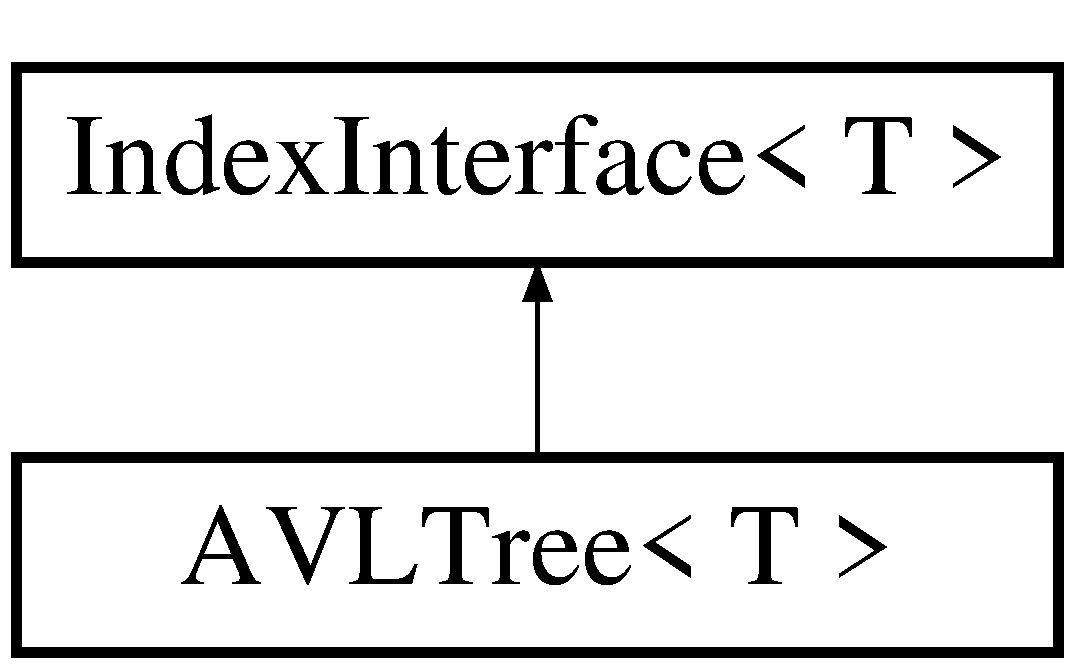
\includegraphics[height=2.000000cm]{classAVLTree}
\end{center}
\end{figure}
\subsection*{Public Member Functions}
\begin{DoxyCompactItemize}
\item 
\mbox{\Hypertarget{classAVLTree_ae060c99e3cbf028cf2cc3dbae477baeb}\label{classAVLTree_ae060c99e3cbf028cf2cc3dbae477baeb}} 
{\bfseries A\+V\+L\+Tree} (const \mbox{\hyperlink{classAVLTree}{A\+V\+L\+Tree}}$<$ T $>$ \&)
\item 
\mbox{\Hypertarget{classAVLTree_a323cd174756feb69b5e164d712bfc13f}\label{classAVLTree_a323cd174756feb69b5e164d712bfc13f}} 
\mbox{\hyperlink{classAVLTree}{A\+V\+L\+Tree}}$<$ T $>$ \& {\bfseries operator=} (const \mbox{\hyperlink{classAVLTree}{A\+V\+L\+Tree}}$<$ T $>$ \&)
\item 
bool \mbox{\hyperlink{classAVLTree_afe724de4c687945d687d7013f4447d20}{contains}} (const T \&) const
\item 
std\+::pair$<$ T, bool $>$ \mbox{\hyperlink{classAVLTree_abc89056d84bd8b7f625f0716788154fb}{search}} (const T \&)
\item 
void \mbox{\hyperlink{classAVLTree_a5b8d9bac5800aec72c175c74391f7027}{insert}} (const T \&)
\item 
bool \mbox{\hyperlink{classAVLTree_a0203b5672172acbb9085d75f37fb674e}{is\+Empty}} () const
\item 
void \mbox{\hyperlink{classAVLTree_ab7062b17bcc409f0b9200671482fad01}{make\+Empty}} ()
\item 
std\+::pair$<$ T, bool $>$ \mbox{\hyperlink{classAVLTree_a2564e8382d86688fca442f3ef960612d}{string\+Search}} (const std\+::string \&)
\item 
void \mbox{\hyperlink{classAVLTree_a241b96e4c35403cabdc44c4781326721}{string\+Insert}} (const std\+::string \&, int, int, int)
\item 
T \& \mbox{\hyperlink{classAVLTree_a2bae23bdf0a05bdfa8c7b77ea46b5d3e}{find\+Max}} ()
\item 
T \& \mbox{\hyperlink{classAVLTree_a3cb9a9b85e4955d79e706f2e589dfc70}{find\+Min}} ()
\item 
std\+::ostream \& \mbox{\hyperlink{classAVLTree_af5299ff77e912f72481679bf9f380810}{print}} (std\+::ostream \&) const
\item 
\mbox{\Hypertarget{classAVLTree_afe1878e13d4f856c915cee90dfd60f86}\label{classAVLTree_afe1878e13d4f856c915cee90dfd60f86}} 
std\+::vector$<$ T $>$ {\bfseries get\+Top\+Fifty} ()
\item 
int \mbox{\hyperlink{classAVLTree_aef337841336fe9e42e4575283139b205}{get\+Terms}} () const
\end{DoxyCompactItemize}
\subsection*{Friends}
\begin{DoxyCompactItemize}
\item 
\mbox{\Hypertarget{classAVLTree_ab87e89a876f46efe5d304239c352e804}\label{classAVLTree_ab87e89a876f46efe5d304239c352e804}} 
{\footnotesize template$<$class U $>$ }\\std\+::ostream \& {\bfseries operator$<$$<$} (std\+::ostream \&, const \mbox{\hyperlink{classAVLTree}{A\+V\+L\+Tree}}$<$ U $>$ \&)
\end{DoxyCompactItemize}


\subsection{Detailed Description}
\subsubsection*{template$<$class T$>$\newline
class A\+V\+L\+Tree$<$ T $>$}

Implements an ordered index as a self-\/balancing A\+VL binary tree.

Also assumes that any values passed in are unique or can have data appended to them with operator+= without changing their ordering. 

\subsection{Member Function Documentation}
\mbox{\Hypertarget{classAVLTree_afe724de4c687945d687d7013f4447d20}\label{classAVLTree_afe724de4c687945d687d7013f4447d20}} 
\index{A\+V\+L\+Tree@{A\+V\+L\+Tree}!contains@{contains}}
\index{contains@{contains}!A\+V\+L\+Tree@{A\+V\+L\+Tree}}
\subsubsection{\texorpdfstring{contains()}{contains()}}
{\footnotesize\ttfamily template$<$class T $>$ \\
bool \mbox{\hyperlink{classAVLTree}{A\+V\+L\+Tree}}$<$ T $>$\+::contains (\begin{DoxyParamCaption}\item[{const T \&}]{arg }\end{DoxyParamCaption}) const\hspace{0.3cm}{\ttfamily [virtual]}}

Determines whether or not the passed argument is an element of the tree 

Implements \mbox{\hyperlink{classIndexInterface}{Index\+Interface$<$ T $>$}}.

\mbox{\Hypertarget{classAVLTree_a2bae23bdf0a05bdfa8c7b77ea46b5d3e}\label{classAVLTree_a2bae23bdf0a05bdfa8c7b77ea46b5d3e}} 
\index{A\+V\+L\+Tree@{A\+V\+L\+Tree}!find\+Max@{find\+Max}}
\index{find\+Max@{find\+Max}!A\+V\+L\+Tree@{A\+V\+L\+Tree}}
\subsubsection{\texorpdfstring{find\+Max()}{findMax()}}
{\footnotesize\ttfamily template$<$class T $>$ \\
T \& \mbox{\hyperlink{classAVLTree}{A\+V\+L\+Tree}}$<$ T $>$\+::find\+Max (\begin{DoxyParamCaption}{ }\end{DoxyParamCaption})}

Returns the maximum value contained in the tree. \mbox{\Hypertarget{classAVLTree_a3cb9a9b85e4955d79e706f2e589dfc70}\label{classAVLTree_a3cb9a9b85e4955d79e706f2e589dfc70}} 
\index{A\+V\+L\+Tree@{A\+V\+L\+Tree}!find\+Min@{find\+Min}}
\index{find\+Min@{find\+Min}!A\+V\+L\+Tree@{A\+V\+L\+Tree}}
\subsubsection{\texorpdfstring{find\+Min()}{findMin()}}
{\footnotesize\ttfamily template$<$class T $>$ \\
T \& \mbox{\hyperlink{classAVLTree}{A\+V\+L\+Tree}}$<$ T $>$\+::find\+Min (\begin{DoxyParamCaption}{ }\end{DoxyParamCaption})}

Returns the minimum value contained in the tree. \mbox{\Hypertarget{classAVLTree_aef337841336fe9e42e4575283139b205}\label{classAVLTree_aef337841336fe9e42e4575283139b205}} 
\index{A\+V\+L\+Tree@{A\+V\+L\+Tree}!get\+Terms@{get\+Terms}}
\index{get\+Terms@{get\+Terms}!A\+V\+L\+Tree@{A\+V\+L\+Tree}}
\subsubsection{\texorpdfstring{get\+Terms()}{getTerms()}}
{\footnotesize\ttfamily template$<$class T $>$ \\
int \mbox{\hyperlink{classAVLTree}{A\+V\+L\+Tree}}$<$ T $>$\+::get\+Terms (\begin{DoxyParamCaption}{ }\end{DoxyParamCaption}) const\hspace{0.3cm}{\ttfamily [virtual]}}

Returns the number of terms that have been indexed by the tree 

Implements \mbox{\hyperlink{classIndexInterface}{Index\+Interface$<$ T $>$}}.

\mbox{\Hypertarget{classAVLTree_a5b8d9bac5800aec72c175c74391f7027}\label{classAVLTree_a5b8d9bac5800aec72c175c74391f7027}} 
\index{A\+V\+L\+Tree@{A\+V\+L\+Tree}!insert@{insert}}
\index{insert@{insert}!A\+V\+L\+Tree@{A\+V\+L\+Tree}}
\subsubsection{\texorpdfstring{insert()}{insert()}}
{\footnotesize\ttfamily template$<$class T $>$ \\
void \mbox{\hyperlink{classAVLTree}{A\+V\+L\+Tree}}$<$ T $>$\+::insert (\begin{DoxyParamCaption}\item[{const T \&}]{arg }\end{DoxyParamCaption})\hspace{0.3cm}{\ttfamily [virtual]}}

Determines where a passed value should be inserted into the tree and inserts there. 

Implements \mbox{\hyperlink{classIndexInterface}{Index\+Interface$<$ T $>$}}.

\mbox{\Hypertarget{classAVLTree_a0203b5672172acbb9085d75f37fb674e}\label{classAVLTree_a0203b5672172acbb9085d75f37fb674e}} 
\index{A\+V\+L\+Tree@{A\+V\+L\+Tree}!is\+Empty@{is\+Empty}}
\index{is\+Empty@{is\+Empty}!A\+V\+L\+Tree@{A\+V\+L\+Tree}}
\subsubsection{\texorpdfstring{is\+Empty()}{isEmpty()}}
{\footnotesize\ttfamily template$<$class T $>$ \\
bool \mbox{\hyperlink{classAVLTree}{A\+V\+L\+Tree}}$<$ T $>$\+::is\+Empty (\begin{DoxyParamCaption}{ }\end{DoxyParamCaption}) const\hspace{0.3cm}{\ttfamily [virtual]}}

Returns true if tree is empty, false if not. 

Implements \mbox{\hyperlink{classIndexInterface}{Index\+Interface$<$ T $>$}}.

\mbox{\Hypertarget{classAVLTree_ab7062b17bcc409f0b9200671482fad01}\label{classAVLTree_ab7062b17bcc409f0b9200671482fad01}} 
\index{A\+V\+L\+Tree@{A\+V\+L\+Tree}!make\+Empty@{make\+Empty}}
\index{make\+Empty@{make\+Empty}!A\+V\+L\+Tree@{A\+V\+L\+Tree}}
\subsubsection{\texorpdfstring{make\+Empty()}{makeEmpty()}}
{\footnotesize\ttfamily template$<$class T $>$ \\
void \mbox{\hyperlink{classAVLTree}{A\+V\+L\+Tree}}$<$ T $>$\+::make\+Empty (\begin{DoxyParamCaption}{ }\end{DoxyParamCaption})\hspace{0.3cm}{\ttfamily [virtual]}}

Empties the tree and frees all allocated memory 

Implements \mbox{\hyperlink{classIndexInterface}{Index\+Interface$<$ T $>$}}.

\mbox{\Hypertarget{classAVLTree_af5299ff77e912f72481679bf9f380810}\label{classAVLTree_af5299ff77e912f72481679bf9f380810}} 
\index{A\+V\+L\+Tree@{A\+V\+L\+Tree}!print@{print}}
\index{print@{print}!A\+V\+L\+Tree@{A\+V\+L\+Tree}}
\subsubsection{\texorpdfstring{print()}{print()}}
{\footnotesize\ttfamily template$<$class T $>$ \\
std\+::ostream \& \mbox{\hyperlink{classAVLTree}{A\+V\+L\+Tree}}$<$ T $>$\+::print (\begin{DoxyParamCaption}\item[{std\+::ostream \&}]{os }\end{DoxyParamCaption}) const\hspace{0.3cm}{\ttfamily [virtual]}}

Prints contents of the tree according to a level-\/order traversal 

Reimplemented from \mbox{\hyperlink{classIndexInterface}{Index\+Interface$<$ T $>$}}.

\mbox{\Hypertarget{classAVLTree_abc89056d84bd8b7f625f0716788154fb}\label{classAVLTree_abc89056d84bd8b7f625f0716788154fb}} 
\index{A\+V\+L\+Tree@{A\+V\+L\+Tree}!search@{search}}
\index{search@{search}!A\+V\+L\+Tree@{A\+V\+L\+Tree}}
\subsubsection{\texorpdfstring{search()}{search()}}
{\footnotesize\ttfamily template$<$class T $>$ \\
std\+::pair$<$ T, bool $>$ \mbox{\hyperlink{classAVLTree}{A\+V\+L\+Tree}}$<$ T $>$\+::search (\begin{DoxyParamCaption}\item[{const T \&}]{arg }\end{DoxyParamCaption})\hspace{0.3cm}{\ttfamily [virtual]}}

Searches for the passed value and returns that data from the tree if it is there. If not, indicates with a false value. 

Implements \mbox{\hyperlink{classIndexInterface}{Index\+Interface$<$ T $>$}}.

\mbox{\Hypertarget{classAVLTree_a241b96e4c35403cabdc44c4781326721}\label{classAVLTree_a241b96e4c35403cabdc44c4781326721}} 
\index{A\+V\+L\+Tree@{A\+V\+L\+Tree}!string\+Insert@{string\+Insert}}
\index{string\+Insert@{string\+Insert}!A\+V\+L\+Tree@{A\+V\+L\+Tree}}
\subsubsection{\texorpdfstring{string\+Insert()}{stringInsert()}}
{\footnotesize\ttfamily template$<$class T $>$ \\
void \mbox{\hyperlink{classAVLTree}{A\+V\+L\+Tree}}$<$ T $>$\+::string\+Insert (\begin{DoxyParamCaption}\item[{const std\+::string \&}]{word,  }\item[{int}]{id,  }\item[{int}]{freq,  }\item[{int}]{loc }\end{DoxyParamCaption})\hspace{0.3cm}{\ttfamily [virtual]}}

Inserts a string to the index based on its string key 

Implements \mbox{\hyperlink{classIndexInterface}{Index\+Interface$<$ T $>$}}.

\mbox{\Hypertarget{classAVLTree_a2564e8382d86688fca442f3ef960612d}\label{classAVLTree_a2564e8382d86688fca442f3ef960612d}} 
\index{A\+V\+L\+Tree@{A\+V\+L\+Tree}!string\+Search@{string\+Search}}
\index{string\+Search@{string\+Search}!A\+V\+L\+Tree@{A\+V\+L\+Tree}}
\subsubsection{\texorpdfstring{string\+Search()}{stringSearch()}}
{\footnotesize\ttfamily template$<$class T $>$ \\
std\+::pair$<$ T, bool $>$ \mbox{\hyperlink{classAVLTree}{A\+V\+L\+Tree}}$<$ T $>$\+::string\+Search (\begin{DoxyParamCaption}\item[{const std\+::string \&}]{word }\end{DoxyParamCaption})\hspace{0.3cm}{\ttfamily [virtual]}}

Searches the tree for Indexed\+Terms based on their string keys 

Implements \mbox{\hyperlink{classIndexInterface}{Index\+Interface$<$ T $>$}}.



The documentation for this class was generated from the following file\+:\begin{DoxyCompactItemize}
\item 
avltree.\+hpp\end{DoxyCompactItemize}

\hypertarget{structCsvParser}{}\section{Csv\+Parser Struct Reference}
\label{structCsvParser}\index{Csv\+Parser@{Csv\+Parser}}
\subsection*{Public Attributes}
\begin{DoxyCompactItemize}
\item 
\mbox{\Hypertarget{structCsvParser_ab6554b8a9f6eb30ab3d70260978e2ba9}\label{structCsvParser_ab6554b8a9f6eb30ab3d70260978e2ba9}} 
char $\ast$ {\bfseries file\+Path\+\_\+}
\item 
\mbox{\Hypertarget{structCsvParser_a2397568bbb5ba5c07f851b3d4912f90a}\label{structCsvParser_a2397568bbb5ba5c07f851b3d4912f90a}} 
char {\bfseries delimiter\+\_\+}
\item 
\mbox{\Hypertarget{structCsvParser_a8ff87dcccef7bf07fc895d346cd06a0b}\label{structCsvParser_a8ff87dcccef7bf07fc895d346cd06a0b}} 
int {\bfseries first\+Line\+Is\+Header\+\_\+}
\item 
\mbox{\Hypertarget{structCsvParser_a94c89d1b1eee9cbbc27229e474fb64b7}\label{structCsvParser_a94c89d1b1eee9cbbc27229e474fb64b7}} 
char $\ast$ {\bfseries err\+Msg\+\_\+}
\item 
\mbox{\Hypertarget{structCsvParser_a874fa706960fbcc1ae2402e6431c31b8}\label{structCsvParser_a874fa706960fbcc1ae2402e6431c31b8}} 
\mbox{\hyperlink{structCsvRow}{Csv\+Row}} $\ast$ {\bfseries header\+\_\+}
\item 
\mbox{\Hypertarget{structCsvParser_a864123b6641654026eea1d8246f48f45}\label{structCsvParser_a864123b6641654026eea1d8246f48f45}} 
F\+I\+LE $\ast$ {\bfseries file\+Handler\+\_\+}
\item 
\mbox{\Hypertarget{structCsvParser_a945f8746ca5d78a43490d44cf3d8b11e}\label{structCsvParser_a945f8746ca5d78a43490d44cf3d8b11e}} 
int {\bfseries from\+String\+\_\+}
\item 
\mbox{\Hypertarget{structCsvParser_acce5ca1892320db4dad5bdb8222b69bf}\label{structCsvParser_acce5ca1892320db4dad5bdb8222b69bf}} 
char $\ast$ {\bfseries csv\+String\+\_\+}
\item 
\mbox{\Hypertarget{structCsvParser_a7f7232b9244877392c4397245f8c55ba}\label{structCsvParser_a7f7232b9244877392c4397245f8c55ba}} 
int {\bfseries csv\+String\+Iter\+\_\+}
\end{DoxyCompactItemize}


The documentation for this struct was generated from the following file\+:\begin{DoxyCompactItemize}
\item 
csvparser.\+h\end{DoxyCompactItemize}

\hypertarget{structCsvRow}{}\section{Csv\+Row Struct Reference}
\label{structCsvRow}\index{Csv\+Row@{Csv\+Row}}
\subsection*{Public Attributes}
\begin{DoxyCompactItemize}
\item 
\mbox{\Hypertarget{structCsvRow_ab59e5601a0ed7ba9b314a2f72088d20b}\label{structCsvRow_ab59e5601a0ed7ba9b314a2f72088d20b}} 
char $\ast$$\ast$ {\bfseries fields\+\_\+}
\item 
\mbox{\Hypertarget{structCsvRow_aad64d8312598aa6b1cea306d7b48dfd3}\label{structCsvRow_aad64d8312598aa6b1cea306d7b48dfd3}} 
int {\bfseries num\+Of\+Fields\+\_\+}
\end{DoxyCompactItemize}


The documentation for this struct was generated from the following file\+:\begin{DoxyCompactItemize}
\item 
csvparser.\+h\end{DoxyCompactItemize}

\hypertarget{classDocumentParser}{}\section{Document\+Parser Class Reference}
\label{classDocumentParser}\index{Document\+Parser@{Document\+Parser}}
\subsection*{Public Member Functions}
\begin{DoxyCompactItemize}
\item 
\mbox{\hyperlink{classDocumentParser_aa038283709a41bc286ae70593ece76ee}{Document\+Parser}} (\mbox{\hyperlink{classIndexHandler}{Index\+Handler}} $\ast$ih)
\begin{DoxyCompactList}\small\item\em Constructor for \mbox{\hyperlink{classDocumentParser}{Document\+Parser}}. \end{DoxyCompactList}\item 
void \mbox{\hyperlink{classDocumentParser_aa385067d0e336601c422b6d64c664d39}{parse}} (std\+::string file\+Name)
\begin{DoxyCompactList}\small\item\em Parses .csv file and seperates fields into an array. \end{DoxyCompactList}\item 
void \mbox{\hyperlink{classDocumentParser_ae192e81639f4473998277136b3a821e5}{load\+Stop\+Words}} (std\+::string file\+Name)
\begin{DoxyCompactList}\small\item\em Loads stop words from file and stores them in set. \end{DoxyCompactList}\item 
std\+::vector$<$ std\+::string $>$ \mbox{\hyperlink{classDocumentParser_a957a602ad41470adfc310f9f16d7c5e7}{question\+Lookup}} (int lookup\+ID, std\+::string document\+Path)
\end{DoxyCompactItemize}


\subsection{Constructor \& Destructor Documentation}
\mbox{\Hypertarget{classDocumentParser_aa038283709a41bc286ae70593ece76ee}\label{classDocumentParser_aa038283709a41bc286ae70593ece76ee}} 
\index{Document\+Parser@{Document\+Parser}!Document\+Parser@{Document\+Parser}}
\index{Document\+Parser@{Document\+Parser}!Document\+Parser@{Document\+Parser}}
\subsubsection{\texorpdfstring{Document\+Parser()}{DocumentParser()}}
{\footnotesize\ttfamily Document\+Parser\+::\+Document\+Parser (\begin{DoxyParamCaption}\item[{\mbox{\hyperlink{classIndexHandler}{Index\+Handler}} $\ast$}]{ih }\end{DoxyParamCaption})}



Constructor for \mbox{\hyperlink{classDocumentParser}{Document\+Parser}}. 


\begin{DoxyParams}{Parameters}
{\em Reference} & to index handler for adding words to an index \\
\hline
\end{DoxyParams}


\subsection{Member Function Documentation}
\mbox{\Hypertarget{classDocumentParser_ae192e81639f4473998277136b3a821e5}\label{classDocumentParser_ae192e81639f4473998277136b3a821e5}} 
\index{Document\+Parser@{Document\+Parser}!load\+Stop\+Words@{load\+Stop\+Words}}
\index{load\+Stop\+Words@{load\+Stop\+Words}!Document\+Parser@{Document\+Parser}}
\subsubsection{\texorpdfstring{load\+Stop\+Words()}{loadStopWords()}}
{\footnotesize\ttfamily void Document\+Parser\+::load\+Stop\+Words (\begin{DoxyParamCaption}\item[{std\+::string}]{file\+Name }\end{DoxyParamCaption})}



Loads stop words from file and stores them in set. 


\begin{DoxyParams}{Parameters}
{\em Name} & of file \\
\hline
\end{DoxyParams}
\mbox{\Hypertarget{classDocumentParser_aa385067d0e336601c422b6d64c664d39}\label{classDocumentParser_aa385067d0e336601c422b6d64c664d39}} 
\index{Document\+Parser@{Document\+Parser}!parse@{parse}}
\index{parse@{parse}!Document\+Parser@{Document\+Parser}}
\subsubsection{\texorpdfstring{parse()}{parse()}}
{\footnotesize\ttfamily void Document\+Parser\+::parse (\begin{DoxyParamCaption}\item[{std\+::string}]{file\+Name }\end{DoxyParamCaption})}



Parses .csv file and seperates fields into an array. 


\begin{DoxyParams}{Parameters}
{\em Name} & of file \\
\hline
\end{DoxyParams}
\mbox{\Hypertarget{classDocumentParser_a957a602ad41470adfc310f9f16d7c5e7}\label{classDocumentParser_a957a602ad41470adfc310f9f16d7c5e7}} 
\index{Document\+Parser@{Document\+Parser}!question\+Lookup@{question\+Lookup}}
\index{question\+Lookup@{question\+Lookup}!Document\+Parser@{Document\+Parser}}
\subsubsection{\texorpdfstring{question\+Lookup()}{questionLookup()}}
{\footnotesize\ttfamily std\+::vector$<$ std\+::string $>$ Document\+Parser\+::question\+Lookup (\begin{DoxyParamCaption}\item[{int}]{lookup\+ID,  }\item[{std\+::string}]{document\+Path }\end{DoxyParamCaption})}

Takes in file path and an ID to be searched and returns question information. Question information is returned as a vector. User needs to be prompted for path to document 

The documentation for this class was generated from the following files\+:\begin{DoxyCompactItemize}
\item 
documentparser.\+h\item 
documentparser.\+cpp\end{DoxyCompactItemize}

\hypertarget{classHashTable}{}\section{Hash\+Table$<$ T $>$ Class Template Reference}
\label{classHashTable}\index{Hash\+Table$<$ T $>$@{Hash\+Table$<$ T $>$}}
Inheritance diagram for Hash\+Table$<$ T $>$\+:\begin{figure}[H]
\begin{center}
\leavevmode
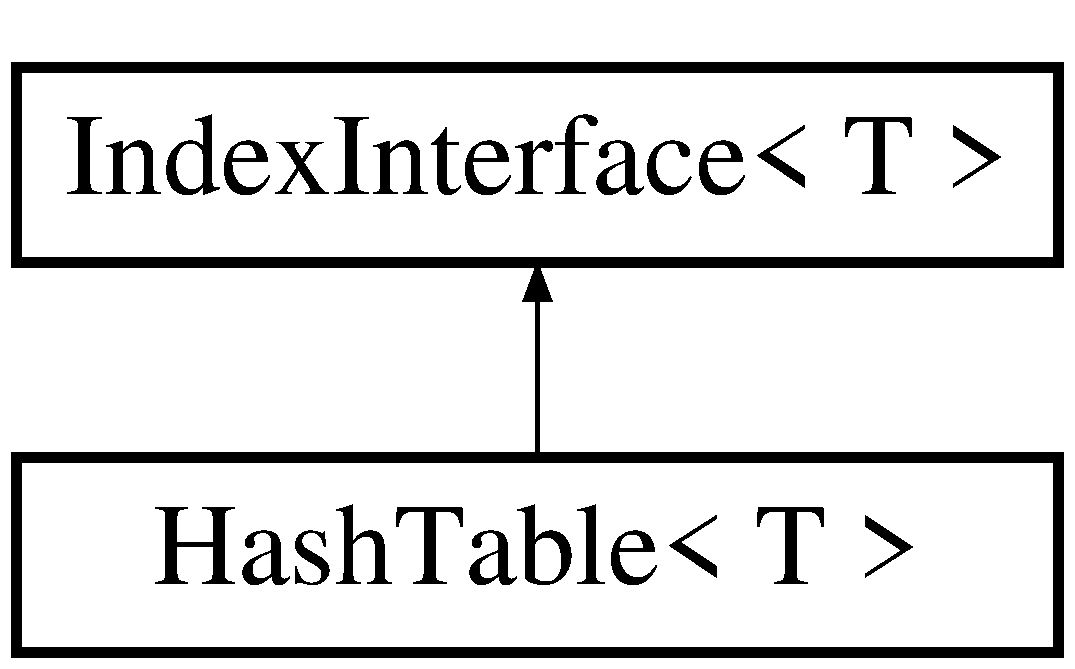
\includegraphics[height=2.000000cm]{classHashTable}
\end{center}
\end{figure}
\subsection*{Public Member Functions}
\begin{DoxyCompactItemize}
\item 
\mbox{\hyperlink{classHashTable_aaf597eeb450b75345dc8ec5061429d66}{Hash\+Table}} (int=1000000)
\item 
\mbox{\hyperlink{classHashTable_a4acb9708dd46d79a1a2aa45a64977a8b}{Hash\+Table}} (const \mbox{\hyperlink{classHashTable}{Hash\+Table}}$<$ T $>$ \&)
\item 
\mbox{\hyperlink{classHashTable}{Hash\+Table}}$<$ T $>$ \& \mbox{\hyperlink{classHashTable_a7db250d46e886751910efdb0e0ac7aad}{operator=}} (const \mbox{\hyperlink{classHashTable}{Hash\+Table}}$<$ T $>$ \&)
\item 
bool \mbox{\hyperlink{classHashTable_ae30d145ec5047b093d27b7b7038a45fa}{contains}} (const T \&) const
\item 
std\+::pair$<$ T, bool $>$ \mbox{\hyperlink{classHashTable_abcc2c56c62a636f9163d934aa6881c57}{search}} (const T \&)
\item 
void \mbox{\hyperlink{classHashTable_a678593aba9238850142914bca5f97158}{insert}} (const T \&)
\item 
bool \mbox{\hyperlink{classHashTable_a3e2bab230f4dd25ba9510f49c5be2b36}{is\+Empty}} () const
\item 
void \mbox{\hyperlink{classHashTable_aaed86109363c5412e7aeebeb0200fe44}{make\+Empty}} ()
\item 
std\+::pair$<$ T, bool $>$ \mbox{\hyperlink{classHashTable_a801997e4fd99d4054bbdff4002e6e63d}{string\+Search}} (const std\+::string \&)
\item 
void \mbox{\hyperlink{classHashTable_a48094fe05d264dcc5f2292b8ca7e2a4c}{string\+Insert}} (const std\+::string \&, int, int, int)
\item 
std\+::ostream \& \mbox{\hyperlink{classHashTable_a925e5d133027e366e6a05d584a04a92c}{print}} (std\+::ostream \&os) const
\item 
int \mbox{\hyperlink{classHashTable_a8b8869f3dc1b79fd2c4fb6488a44926c}{get\+Num\+Elements}} () const
\item 
std\+::pair$<$ T, bool $>$ \mbox{\hyperlink{classHashTable_a97088b8890aa3ef1403359d45b6260ce}{operator\mbox{[}$\,$\mbox{]}}} (const T \&)
\item 
std\+::vector$<$ T $>$ \mbox{\hyperlink{classHashTable_a6f5359b3b5b29414ef07fcb202b0ed28}{get\+Top\+Fifty}} ()
\item 
int \mbox{\hyperlink{classHashTable_a1da70d706b97754c2bd359d2f512b087}{get\+Terms}} () const
\end{DoxyCompactItemize}
\subsection*{Friends}
\begin{DoxyCompactItemize}
\item 
\mbox{\Hypertarget{classHashTable_aedd40d8c02fdaf28f43533eefff0e4f4}\label{classHashTable_aedd40d8c02fdaf28f43533eefff0e4f4}} 
{\footnotesize template$<$class U $>$ }\\std\+::ostream \& {\bfseries operator$<$$<$} (std\+::ostream \&, const \mbox{\hyperlink{classHashTable}{Hash\+Table}}$<$ U $>$ \&)
\end{DoxyCompactItemize}


\subsection{Constructor \& Destructor Documentation}
\mbox{\Hypertarget{classHashTable_aaf597eeb450b75345dc8ec5061429d66}\label{classHashTable_aaf597eeb450b75345dc8ec5061429d66}} 
\index{Hash\+Table@{Hash\+Table}!Hash\+Table@{Hash\+Table}}
\index{Hash\+Table@{Hash\+Table}!Hash\+Table@{Hash\+Table}}
\subsubsection{\texorpdfstring{Hash\+Table()}{HashTable()}\hspace{0.1cm}{\footnotesize\ttfamily [1/2]}}
{\footnotesize\ttfamily template$<$class T $>$ \\
\mbox{\hyperlink{classHashTable}{Hash\+Table}}$<$ T $>$\+::\mbox{\hyperlink{classHashTable}{Hash\+Table}} (\begin{DoxyParamCaption}\item[{int}]{size = {\ttfamily 1000000} }\end{DoxyParamCaption})}

Default constructor initializes array \mbox{\Hypertarget{classHashTable_a4acb9708dd46d79a1a2aa45a64977a8b}\label{classHashTable_a4acb9708dd46d79a1a2aa45a64977a8b}} 
\index{Hash\+Table@{Hash\+Table}!Hash\+Table@{Hash\+Table}}
\index{Hash\+Table@{Hash\+Table}!Hash\+Table@{Hash\+Table}}
\subsubsection{\texorpdfstring{Hash\+Table()}{HashTable()}\hspace{0.1cm}{\footnotesize\ttfamily [2/2]}}
{\footnotesize\ttfamily template$<$class T $>$ \\
\mbox{\hyperlink{classHashTable}{Hash\+Table}}$<$ T $>$\+::\mbox{\hyperlink{classHashTable}{Hash\+Table}} (\begin{DoxyParamCaption}\item[{const \mbox{\hyperlink{classHashTable}{Hash\+Table}}$<$ T $>$ \&}]{rhs }\end{DoxyParamCaption})}

Copy constructor copies over elements of vector 

\subsection{Member Function Documentation}
\mbox{\Hypertarget{classHashTable_ae30d145ec5047b093d27b7b7038a45fa}\label{classHashTable_ae30d145ec5047b093d27b7b7038a45fa}} 
\index{Hash\+Table@{Hash\+Table}!contains@{contains}}
\index{contains@{contains}!Hash\+Table@{Hash\+Table}}
\subsubsection{\texorpdfstring{contains()}{contains()}}
{\footnotesize\ttfamily template$<$class T $>$ \\
bool \mbox{\hyperlink{classHashTable}{Hash\+Table}}$<$ T $>$\+::contains (\begin{DoxyParamCaption}\item[{const T \&}]{to\+Be\+Found }\end{DoxyParamCaption}) const\hspace{0.3cm}{\ttfamily [virtual]}}

Determines whether or not the table contains the given argument 

Implements \mbox{\hyperlink{classIndexInterface}{Index\+Interface$<$ T $>$}}.

\mbox{\Hypertarget{classHashTable_a8b8869f3dc1b79fd2c4fb6488a44926c}\label{classHashTable_a8b8869f3dc1b79fd2c4fb6488a44926c}} 
\index{Hash\+Table@{Hash\+Table}!get\+Num\+Elements@{get\+Num\+Elements}}
\index{get\+Num\+Elements@{get\+Num\+Elements}!Hash\+Table@{Hash\+Table}}
\subsubsection{\texorpdfstring{get\+Num\+Elements()}{getNumElements()}}
{\footnotesize\ttfamily template$<$class T $>$ \\
int \mbox{\hyperlink{classHashTable}{Hash\+Table}}$<$ T $>$\+::get\+Num\+Elements (\begin{DoxyParamCaption}{ }\end{DoxyParamCaption}) const}

Returns the number of elements in the table \mbox{\Hypertarget{classHashTable_a1da70d706b97754c2bd359d2f512b087}\label{classHashTable_a1da70d706b97754c2bd359d2f512b087}} 
\index{Hash\+Table@{Hash\+Table}!get\+Terms@{get\+Terms}}
\index{get\+Terms@{get\+Terms}!Hash\+Table@{Hash\+Table}}
\subsubsection{\texorpdfstring{get\+Terms()}{getTerms()}}
{\footnotesize\ttfamily template$<$class T $>$ \\
int \mbox{\hyperlink{classHashTable}{Hash\+Table}}$<$ T $>$\+::get\+Terms (\begin{DoxyParamCaption}{ }\end{DoxyParamCaption}) const\hspace{0.3cm}{\ttfamily [virtual]}}

Returns the number of elements indexed by the table 

Implements \mbox{\hyperlink{classIndexInterface}{Index\+Interface$<$ T $>$}}.

\mbox{\Hypertarget{classHashTable_a6f5359b3b5b29414ef07fcb202b0ed28}\label{classHashTable_a6f5359b3b5b29414ef07fcb202b0ed28}} 
\index{Hash\+Table@{Hash\+Table}!get\+Top\+Fifty@{get\+Top\+Fifty}}
\index{get\+Top\+Fifty@{get\+Top\+Fifty}!Hash\+Table@{Hash\+Table}}
\subsubsection{\texorpdfstring{get\+Top\+Fifty()}{getTopFifty()}}
{\footnotesize\ttfamily template$<$class T $>$ \\
std\+::vector$<$ T $>$ \mbox{\hyperlink{classHashTable}{Hash\+Table}}$<$ T $>$\+::get\+Top\+Fifty (\begin{DoxyParamCaption}{ }\end{DoxyParamCaption})\hspace{0.3cm}{\ttfamily [virtual]}}

Returns a vector of the top fifty most common sords. 

Implements \mbox{\hyperlink{classIndexInterface}{Index\+Interface$<$ T $>$}}.

\mbox{\Hypertarget{classHashTable_a678593aba9238850142914bca5f97158}\label{classHashTable_a678593aba9238850142914bca5f97158}} 
\index{Hash\+Table@{Hash\+Table}!insert@{insert}}
\index{insert@{insert}!Hash\+Table@{Hash\+Table}}
\subsubsection{\texorpdfstring{insert()}{insert()}}
{\footnotesize\ttfamily template$<$class T $>$ \\
void \mbox{\hyperlink{classHashTable}{Hash\+Table}}$<$ T $>$\+::insert (\begin{DoxyParamCaption}\item[{const T \&}]{inserted }\end{DoxyParamCaption})\hspace{0.3cm}{\ttfamily [virtual]}}

Inserts new object to position given by hashing function 

Implements \mbox{\hyperlink{classIndexInterface}{Index\+Interface$<$ T $>$}}.

\mbox{\Hypertarget{classHashTable_a3e2bab230f4dd25ba9510f49c5be2b36}\label{classHashTable_a3e2bab230f4dd25ba9510f49c5be2b36}} 
\index{Hash\+Table@{Hash\+Table}!is\+Empty@{is\+Empty}}
\index{is\+Empty@{is\+Empty}!Hash\+Table@{Hash\+Table}}
\subsubsection{\texorpdfstring{is\+Empty()}{isEmpty()}}
{\footnotesize\ttfamily template$<$class T $>$ \\
bool \mbox{\hyperlink{classHashTable}{Hash\+Table}}$<$ T $>$\+::is\+Empty (\begin{DoxyParamCaption}{ }\end{DoxyParamCaption}) const\hspace{0.3cm}{\ttfamily [virtual]}}

Determines whether or not there are any elements in the table 

Implements \mbox{\hyperlink{classIndexInterface}{Index\+Interface$<$ T $>$}}.

\mbox{\Hypertarget{classHashTable_aaed86109363c5412e7aeebeb0200fe44}\label{classHashTable_aaed86109363c5412e7aeebeb0200fe44}} 
\index{Hash\+Table@{Hash\+Table}!make\+Empty@{make\+Empty}}
\index{make\+Empty@{make\+Empty}!Hash\+Table@{Hash\+Table}}
\subsubsection{\texorpdfstring{make\+Empty()}{makeEmpty()}}
{\footnotesize\ttfamily template$<$class T $>$ \\
void \mbox{\hyperlink{classHashTable}{Hash\+Table}}$<$ T $>$\+::make\+Empty (\begin{DoxyParamCaption}{ }\end{DoxyParamCaption})\hspace{0.3cm}{\ttfamily [virtual]}}

Clears table of all old elements 

Implements \mbox{\hyperlink{classIndexInterface}{Index\+Interface$<$ T $>$}}.

\mbox{\Hypertarget{classHashTable_a7db250d46e886751910efdb0e0ac7aad}\label{classHashTable_a7db250d46e886751910efdb0e0ac7aad}} 
\index{Hash\+Table@{Hash\+Table}!operator=@{operator=}}
\index{operator=@{operator=}!Hash\+Table@{Hash\+Table}}
\subsubsection{\texorpdfstring{operator=()}{operator=()}}
{\footnotesize\ttfamily template$<$class T $>$ \\
\mbox{\hyperlink{classHashTable}{Hash\+Table}}$<$ T $>$ \& \mbox{\hyperlink{classHashTable}{Hash\+Table}}$<$ T $>$\+::operator= (\begin{DoxyParamCaption}\item[{const \mbox{\hyperlink{classHashTable}{Hash\+Table}}$<$ T $>$ \&}]{rhs }\end{DoxyParamCaption})}

Assignment operator copies over data if given argument is not identical \mbox{\Hypertarget{classHashTable_a97088b8890aa3ef1403359d45b6260ce}\label{classHashTable_a97088b8890aa3ef1403359d45b6260ce}} 
\index{Hash\+Table@{Hash\+Table}!operator\mbox{[}\mbox{]}@{operator[]}}
\index{operator\mbox{[}\mbox{]}@{operator[]}!Hash\+Table@{Hash\+Table}}
\subsubsection{\texorpdfstring{operator[]()}{operator[]()}}
{\footnotesize\ttfamily template$<$class T $>$ \\
std\+::pair$<$ T, bool $>$ \mbox{\hyperlink{classHashTable}{Hash\+Table}}$<$ T $>$\+::operator\mbox{[}$\,$\mbox{]} (\begin{DoxyParamCaption}\item[{const T \&}]{sought }\end{DoxyParamCaption})}

Subscript operator accepts argument of type template parameter and returns object stored at that key in the table \mbox{\Hypertarget{classHashTable_a925e5d133027e366e6a05d584a04a92c}\label{classHashTable_a925e5d133027e366e6a05d584a04a92c}} 
\index{Hash\+Table@{Hash\+Table}!print@{print}}
\index{print@{print}!Hash\+Table@{Hash\+Table}}
\subsubsection{\texorpdfstring{print()}{print()}}
{\footnotesize\ttfamily template$<$class T $>$ \\
std\+::ostream \& \mbox{\hyperlink{classHashTable}{Hash\+Table}}$<$ T $>$\+::print (\begin{DoxyParamCaption}\item[{std\+::ostream \&}]{os }\end{DoxyParamCaption}) const\hspace{0.3cm}{\ttfamily [virtual]}}

Prints all elements in table in order of hash value 

Reimplemented from \mbox{\hyperlink{classIndexInterface}{Index\+Interface$<$ T $>$}}.

\mbox{\Hypertarget{classHashTable_abcc2c56c62a636f9163d934aa6881c57}\label{classHashTable_abcc2c56c62a636f9163d934aa6881c57}} 
\index{Hash\+Table@{Hash\+Table}!search@{search}}
\index{search@{search}!Hash\+Table@{Hash\+Table}}
\subsubsection{\texorpdfstring{search()}{search()}}
{\footnotesize\ttfamily template$<$class T $>$ \\
std\+::pair$<$ T, bool $>$ \mbox{\hyperlink{classHashTable}{Hash\+Table}}$<$ T $>$\+::search (\begin{DoxyParamCaption}\item[{const T \&}]{sought }\end{DoxyParamCaption})\hspace{0.3cm}{\ttfamily [virtual]}}

Returns pair with the sought object and a boolean flag indicating whether or not it was found 

Implements \mbox{\hyperlink{classIndexInterface}{Index\+Interface$<$ T $>$}}.

\mbox{\Hypertarget{classHashTable_a48094fe05d264dcc5f2292b8ca7e2a4c}\label{classHashTable_a48094fe05d264dcc5f2292b8ca7e2a4c}} 
\index{Hash\+Table@{Hash\+Table}!string\+Insert@{string\+Insert}}
\index{string\+Insert@{string\+Insert}!Hash\+Table@{Hash\+Table}}
\subsubsection{\texorpdfstring{string\+Insert()}{stringInsert()}}
{\footnotesize\ttfamily template$<$class T $>$ \\
void \mbox{\hyperlink{classHashTable}{Hash\+Table}}$<$ T $>$\+::string\+Insert (\begin{DoxyParamCaption}\item[{const std\+::string \&}]{word,  }\item[{int}]{id,  }\item[{int}]{freq,  }\item[{int}]{loc }\end{DoxyParamCaption})\hspace{0.3cm}{\ttfamily [virtual]}}

Searches for a term matching the given string in the index. If found, appends the data to that term. If not, inserts it to the index. 

Implements \mbox{\hyperlink{classIndexInterface}{Index\+Interface$<$ T $>$}}.

\mbox{\Hypertarget{classHashTable_a801997e4fd99d4054bbdff4002e6e63d}\label{classHashTable_a801997e4fd99d4054bbdff4002e6e63d}} 
\index{Hash\+Table@{Hash\+Table}!string\+Search@{string\+Search}}
\index{string\+Search@{string\+Search}!Hash\+Table@{Hash\+Table}}
\subsubsection{\texorpdfstring{string\+Search()}{stringSearch()}}
{\footnotesize\ttfamily template$<$class T $>$ \\
std\+::pair$<$ T, bool $>$ \mbox{\hyperlink{classHashTable}{Hash\+Table}}$<$ T $>$\+::string\+Search (\begin{DoxyParamCaption}\item[{const std\+::string \&}]{word }\end{DoxyParamCaption})\hspace{0.3cm}{\ttfamily [virtual]}}

Searches the index for an index whose key matches the string passed as argument. 

Implements \mbox{\hyperlink{classIndexInterface}{Index\+Interface$<$ T $>$}}.



The documentation for this class was generated from the following file\+:\begin{DoxyCompactItemize}
\item 
hashtable.\+hpp\end{DoxyCompactItemize}

\hypertarget{classIndexedTerm}{}\section{Indexed\+Term Class Reference}
\label{classIndexedTerm}\index{Indexed\+Term@{Indexed\+Term}}
\subsection*{Public Member Functions}
\begin{DoxyCompactItemize}
\item 
\mbox{\Hypertarget{classIndexedTerm_af4607f12639a14652e3ed27585d636b5}\label{classIndexedTerm_af4607f12639a14652e3ed27585d636b5}} 
{\bfseries Indexed\+Term} (std\+::string=\char`\"{}\char`\"{})
\item 
\mbox{\Hypertarget{classIndexedTerm_ad3ff525566ada45119cc4d044e4733e6}\label{classIndexedTerm_ad3ff525566ada45119cc4d044e4733e6}} 
{\bfseries Indexed\+Term} (std\+::string, int, int, int)
\item 
std\+::string \mbox{\hyperlink{classIndexedTerm_a6e41546c9874e5382b969c41e87c3d8b}{get\+Term}} () const
\item 
bool \mbox{\hyperlink{classIndexedTerm_aeb3a182538b603b10819d6b3310f6747}{is\+Empty}} () const
\item 
int \mbox{\hyperlink{classIndexedTerm_a10df671670e9581f273a7248ca5cbe4b}{get\+Frequency}} (int) const
\item 
std\+::vector$<$ int $>$ \mbox{\hyperlink{classIndexedTerm_a195c332d821640539eadeca10514cc82}{get\+Locations}} (int) const
\item 
std\+::set$<$ int $>$ \mbox{\hyperlink{classIndexedTerm_a585907deff7738139894dd45afa11a63}{get\+Question\+Ids}} () const
\item 
void \mbox{\hyperlink{classIndexedTerm_aa55a9b814c7b084b2e33fb57aa81efaf}{add\+Question}} (int)
\item 
void \mbox{\hyperlink{classIndexedTerm_a766b250a2e276ddd3270e1eb19d1d10d}{remove\+Question}} (int)
\item 
std\+::vector$<$ std\+::pair$<$ int, int $>$ $>$ \mbox{\hyperlink{classIndexedTerm_acbffdf0e7324840c5157ff18f3de67cc}{print15}} ()
\begin{DoxyCompactList}\small\item\em Prints the first 15 values of the sorted Vector of results. \end{DoxyCompactList}\item 
void \mbox{\hyperlink{classIndexedTerm_a923c8542c47170f848610bd7132eb71d}{sort}} (std\+::vector$<$ question\+Index $>$ \&, int)
\item 
\mbox{\Hypertarget{classIndexedTerm_a59228c1c0333e71bc7fbed72aae7cfdf}\label{classIndexedTerm_a59228c1c0333e71bc7fbed72aae7cfdf}} 
\mbox{\hyperlink{classIndexedTerm}{Indexed\+Term}} {\bfseries question\+And} (const \mbox{\hyperlink{classIndexedTerm}{Indexed\+Term}} \&) const
\item 
\mbox{\Hypertarget{classIndexedTerm_a94bc68700a69aa4ef5595c42cacb9aa5}\label{classIndexedTerm_a94bc68700a69aa4ef5595c42cacb9aa5}} 
\mbox{\hyperlink{classIndexedTerm}{Indexed\+Term}} {\bfseries question\+Or} (const \mbox{\hyperlink{classIndexedTerm}{Indexed\+Term}} \&) const
\item 
bool \mbox{\hyperlink{classIndexedTerm_a1b78549f18a68457fcd438ca33d7ab87}{is\+In\+Question}} (int) const
\item 
void \mbox{\hyperlink{classIndexedTerm_acb1a3eebd31bfa50c78ce0371ec7d444}{add\+Location}} (int, int)
\item 
void \mbox{\hyperlink{classIndexedTerm_ac0b5314a66c032780ffcd9d4f9a1d01b}{remove\+Location}} (int, int)
\item 
void \mbox{\hyperlink{classIndexedTerm_a34d9c26b92764dee339e754264bf6343}{add\+Frequency}} (int, int)
\item 
bool \mbox{\hyperlink{classIndexedTerm_ae39f762b1fce474a50bde0a411d34f70}{is\+At\+Location}} (int, int) const
\item 
void \mbox{\hyperlink{classIndexedTerm_ad5b7b07b86c72b049c30204531b5cf53}{append\+Data}} (int, int, int) const
\item 
\mbox{\Hypertarget{classIndexedTerm_ad4db70e1ba7defe2c32e00987635d0b3}\label{classIndexedTerm_ad4db70e1ba7defe2c32e00987635d0b3}} 
int {\bfseries get\+Total\+Freq} () const
\item 
bool \mbox{\hyperlink{classIndexedTerm_ae8a7856cb7afd5b7029df2a47bf3c378}{operator==}} (const \mbox{\hyperlink{classIndexedTerm}{Indexed\+Term}} \&) const
\item 
void \mbox{\hyperlink{classIndexedTerm_a826c10c65c29cb7128e485906f884d31}{operator+=}} (const \mbox{\hyperlink{classIndexedTerm}{Indexed\+Term}} \&) const
\item 
bool \mbox{\hyperlink{classIndexedTerm_a770d1caf59facdb5694493aa57123abb}{operator$>$}} (const \mbox{\hyperlink{classIndexedTerm}{Indexed\+Term}} \&) const
\item 
bool \mbox{\hyperlink{classIndexedTerm_aab009480a31b3f9ab1e1d712cf9f8298}{operator$<$}} (const \mbox{\hyperlink{classIndexedTerm}{Indexed\+Term}} \&) const
\end{DoxyCompactItemize}
\subsection*{Friends}
\begin{DoxyCompactItemize}
\item 
\mbox{\Hypertarget{classIndexedTerm_a56eb771de7ee127bd3a872942ab50d55}\label{classIndexedTerm_a56eb771de7ee127bd3a872942ab50d55}} 
std\+::ostream \& {\bfseries operator$<$$<$} (std\+::ostream \&os, \mbox{\hyperlink{classIndexedTerm}{Indexed\+Term}} it)
\end{DoxyCompactItemize}


\subsection{Member Function Documentation}
\mbox{\Hypertarget{classIndexedTerm_a34d9c26b92764dee339e754264bf6343}\label{classIndexedTerm_a34d9c26b92764dee339e754264bf6343}} 
\index{Indexed\+Term@{Indexed\+Term}!add\+Frequency@{add\+Frequency}}
\index{add\+Frequency@{add\+Frequency}!Indexed\+Term@{Indexed\+Term}}
\subsubsection{\texorpdfstring{add\+Frequency()}{addFrequency()}}
{\footnotesize\ttfamily void Indexed\+Term\+::add\+Frequency (\begin{DoxyParamCaption}\item[{int}]{question\+Id,  }\item[{int}]{frequency }\end{DoxyParamCaption})}

Adds frequency to frequency of specified question \mbox{\Hypertarget{classIndexedTerm_acb1a3eebd31bfa50c78ce0371ec7d444}\label{classIndexedTerm_acb1a3eebd31bfa50c78ce0371ec7d444}} 
\index{Indexed\+Term@{Indexed\+Term}!add\+Location@{add\+Location}}
\index{add\+Location@{add\+Location}!Indexed\+Term@{Indexed\+Term}}
\subsubsection{\texorpdfstring{add\+Location()}{addLocation()}}
{\footnotesize\ttfamily void Indexed\+Term\+::add\+Location (\begin{DoxyParamCaption}\item[{int}]{question\+Id,  }\item[{int}]{location }\end{DoxyParamCaption})}

Adds location to location vector of specified question \mbox{\Hypertarget{classIndexedTerm_aa55a9b814c7b084b2e33fb57aa81efaf}\label{classIndexedTerm_aa55a9b814c7b084b2e33fb57aa81efaf}} 
\index{Indexed\+Term@{Indexed\+Term}!add\+Question@{add\+Question}}
\index{add\+Question@{add\+Question}!Indexed\+Term@{Indexed\+Term}}
\subsubsection{\texorpdfstring{add\+Question()}{addQuestion()}}
{\footnotesize\ttfamily void Indexed\+Term\+::add\+Question (\begin{DoxyParamCaption}\item[{int}]{question\+Id }\end{DoxyParamCaption})}

Adds question\+Id to the set of questions this term is found in. \mbox{\Hypertarget{classIndexedTerm_ad5b7b07b86c72b049c30204531b5cf53}\label{classIndexedTerm_ad5b7b07b86c72b049c30204531b5cf53}} 
\index{Indexed\+Term@{Indexed\+Term}!append\+Data@{append\+Data}}
\index{append\+Data@{append\+Data}!Indexed\+Term@{Indexed\+Term}}
\subsubsection{\texorpdfstring{append\+Data()}{appendData()}}
{\footnotesize\ttfamily void Indexed\+Term\+::append\+Data (\begin{DoxyParamCaption}\item[{int}]{question\+Id,  }\item[{int}]{frequency,  }\item[{int}]{location }\end{DoxyParamCaption}) const}

Appends all data associated with a particular question to the term. \mbox{\Hypertarget{classIndexedTerm_a10df671670e9581f273a7248ca5cbe4b}\label{classIndexedTerm_a10df671670e9581f273a7248ca5cbe4b}} 
\index{Indexed\+Term@{Indexed\+Term}!get\+Frequency@{get\+Frequency}}
\index{get\+Frequency@{get\+Frequency}!Indexed\+Term@{Indexed\+Term}}
\subsubsection{\texorpdfstring{get\+Frequency()}{getFrequency()}}
{\footnotesize\ttfamily int Indexed\+Term\+::get\+Frequency (\begin{DoxyParamCaption}\item[{int}]{question\+ID }\end{DoxyParamCaption}) const}

Retrieves the frequency of the question ID passed as argument; returns 0 if not present. \mbox{\Hypertarget{classIndexedTerm_a195c332d821640539eadeca10514cc82}\label{classIndexedTerm_a195c332d821640539eadeca10514cc82}} 
\index{Indexed\+Term@{Indexed\+Term}!get\+Locations@{get\+Locations}}
\index{get\+Locations@{get\+Locations}!Indexed\+Term@{Indexed\+Term}}
\subsubsection{\texorpdfstring{get\+Locations()}{getLocations()}}
{\footnotesize\ttfamily std\+::vector$<$ int $>$ Indexed\+Term\+::get\+Locations (\begin{DoxyParamCaption}\item[{int}]{question\+Id }\end{DoxyParamCaption}) const}

Returns the vector of locations attached to the given question ID. \mbox{\Hypertarget{classIndexedTerm_a585907deff7738139894dd45afa11a63}\label{classIndexedTerm_a585907deff7738139894dd45afa11a63}} 
\index{Indexed\+Term@{Indexed\+Term}!get\+Question\+Ids@{get\+Question\+Ids}}
\index{get\+Question\+Ids@{get\+Question\+Ids}!Indexed\+Term@{Indexed\+Term}}
\subsubsection{\texorpdfstring{get\+Question\+Ids()}{getQuestionIds()}}
{\footnotesize\ttfamily std\+::set$<$ int $>$ Indexed\+Term\+::get\+Question\+Ids (\begin{DoxyParamCaption}{ }\end{DoxyParamCaption}) const}

Returns a set of all of the question I\+Ds that this term is found in \mbox{\Hypertarget{classIndexedTerm_a6e41546c9874e5382b969c41e87c3d8b}\label{classIndexedTerm_a6e41546c9874e5382b969c41e87c3d8b}} 
\index{Indexed\+Term@{Indexed\+Term}!get\+Term@{get\+Term}}
\index{get\+Term@{get\+Term}!Indexed\+Term@{Indexed\+Term}}
\subsubsection{\texorpdfstring{get\+Term()}{getTerm()}}
{\footnotesize\ttfamily std\+::string Indexed\+Term\+::get\+Term (\begin{DoxyParamCaption}{ }\end{DoxyParamCaption}) const}

Gets value of search term \mbox{\Hypertarget{classIndexedTerm_ae39f762b1fce474a50bde0a411d34f70}\label{classIndexedTerm_ae39f762b1fce474a50bde0a411d34f70}} 
\index{Indexed\+Term@{Indexed\+Term}!is\+At\+Location@{is\+At\+Location}}
\index{is\+At\+Location@{is\+At\+Location}!Indexed\+Term@{Indexed\+Term}}
\subsubsection{\texorpdfstring{is\+At\+Location()}{isAtLocation()}}
{\footnotesize\ttfamily bool Indexed\+Term\+::is\+At\+Location (\begin{DoxyParamCaption}\item[{int}]{question\+Id,  }\item[{int}]{location }\end{DoxyParamCaption}) const}

Determines whether or not the term appears in the given question at the given location. \mbox{\Hypertarget{classIndexedTerm_aeb3a182538b603b10819d6b3310f6747}\label{classIndexedTerm_aeb3a182538b603b10819d6b3310f6747}} 
\index{Indexed\+Term@{Indexed\+Term}!is\+Empty@{is\+Empty}}
\index{is\+Empty@{is\+Empty}!Indexed\+Term@{Indexed\+Term}}
\subsubsection{\texorpdfstring{is\+Empty()}{isEmpty()}}
{\footnotesize\ttfamily bool Indexed\+Term\+::is\+Empty (\begin{DoxyParamCaption}{ }\end{DoxyParamCaption}) const}

Determines whether or not the set of question I\+Ds is empty \mbox{\Hypertarget{classIndexedTerm_a1b78549f18a68457fcd438ca33d7ab87}\label{classIndexedTerm_a1b78549f18a68457fcd438ca33d7ab87}} 
\index{Indexed\+Term@{Indexed\+Term}!is\+In\+Question@{is\+In\+Question}}
\index{is\+In\+Question@{is\+In\+Question}!Indexed\+Term@{Indexed\+Term}}
\subsubsection{\texorpdfstring{is\+In\+Question()}{isInQuestion()}}
{\footnotesize\ttfamily bool Indexed\+Term\+::is\+In\+Question (\begin{DoxyParamCaption}\item[{int}]{question\+Id }\end{DoxyParamCaption}) const}

Returns true if term is in question, false if not \mbox{\Hypertarget{classIndexedTerm_a826c10c65c29cb7128e485906f884d31}\label{classIndexedTerm_a826c10c65c29cb7128e485906f884d31}} 
\index{Indexed\+Term@{Indexed\+Term}!operator+=@{operator+=}}
\index{operator+=@{operator+=}!Indexed\+Term@{Indexed\+Term}}
\subsubsection{\texorpdfstring{operator+=()}{operator+=()}}
{\footnotesize\ttfamily void Indexed\+Term\+::operator+= (\begin{DoxyParamCaption}\item[{const \mbox{\hyperlink{classIndexedTerm}{Indexed\+Term}} \&}]{rhs }\end{DoxyParamCaption}) const}

Addition Assignment Operator adds question ID to list if it isn\textquotesingle{}t there, if it is present, adds frequency \mbox{\Hypertarget{classIndexedTerm_aab009480a31b3f9ab1e1d712cf9f8298}\label{classIndexedTerm_aab009480a31b3f9ab1e1d712cf9f8298}} 
\index{Indexed\+Term@{Indexed\+Term}!operator$<$@{operator$<$}}
\index{operator$<$@{operator$<$}!Indexed\+Term@{Indexed\+Term}}
\subsubsection{\texorpdfstring{operator$<$()}{operator<()}}
{\footnotesize\ttfamily bool Indexed\+Term\+::operator$<$ (\begin{DoxyParamCaption}\item[{const \mbox{\hyperlink{classIndexedTerm}{Indexed\+Term}} \&}]{rhs }\end{DoxyParamCaption}) const}

Compares the terms using lexicographical comparison of the A\+S\+C\+II values of each character in the string. \mbox{\Hypertarget{classIndexedTerm_ae8a7856cb7afd5b7029df2a47bf3c378}\label{classIndexedTerm_ae8a7856cb7afd5b7029df2a47bf3c378}} 
\index{Indexed\+Term@{Indexed\+Term}!operator==@{operator==}}
\index{operator==@{operator==}!Indexed\+Term@{Indexed\+Term}}
\subsubsection{\texorpdfstring{operator==()}{operator==()}}
{\footnotesize\ttfamily bool Indexed\+Term\+::operator== (\begin{DoxyParamCaption}\item[{const \mbox{\hyperlink{classIndexedTerm}{Indexed\+Term}} \&}]{rhs }\end{DoxyParamCaption}) const}

Equality operator checks keys (terms) for equality \mbox{\Hypertarget{classIndexedTerm_a770d1caf59facdb5694493aa57123abb}\label{classIndexedTerm_a770d1caf59facdb5694493aa57123abb}} 
\index{Indexed\+Term@{Indexed\+Term}!operator$>$@{operator$>$}}
\index{operator$>$@{operator$>$}!Indexed\+Term@{Indexed\+Term}}
\subsubsection{\texorpdfstring{operator$>$()}{operator>()}}
{\footnotesize\ttfamily bool Indexed\+Term\+::operator$>$ (\begin{DoxyParamCaption}\item[{const \mbox{\hyperlink{classIndexedTerm}{Indexed\+Term}} \&}]{rhs }\end{DoxyParamCaption}) const}

Compares the terms using lexicographical comparison of the A\+S\+C\+II values of each character in the string. \mbox{\Hypertarget{classIndexedTerm_acbffdf0e7324840c5157ff18f3de67cc}\label{classIndexedTerm_acbffdf0e7324840c5157ff18f3de67cc}} 
\index{Indexed\+Term@{Indexed\+Term}!print15@{print15}}
\index{print15@{print15}!Indexed\+Term@{Indexed\+Term}}
\subsubsection{\texorpdfstring{print15()}{print15()}}
{\footnotesize\ttfamily std\+::vector$<$ std\+::pair$<$ int, int $>$ $>$ Indexed\+Term\+::print15 (\begin{DoxyParamCaption}{ }\end{DoxyParamCaption})}



Prints the first 15 values of the sorted Vector of results. 

\begin{DoxyReturn}{Returns}
a vector of pairs containing question\+I\+Ds and and frequencies of a term 
\end{DoxyReturn}
\mbox{\Hypertarget{classIndexedTerm_ac0b5314a66c032780ffcd9d4f9a1d01b}\label{classIndexedTerm_ac0b5314a66c032780ffcd9d4f9a1d01b}} 
\index{Indexed\+Term@{Indexed\+Term}!remove\+Location@{remove\+Location}}
\index{remove\+Location@{remove\+Location}!Indexed\+Term@{Indexed\+Term}}
\subsubsection{\texorpdfstring{remove\+Location()}{removeLocation()}}
{\footnotesize\ttfamily void Indexed\+Term\+::remove\+Location (\begin{DoxyParamCaption}\item[{int}]{question\+Id,  }\item[{int}]{location }\end{DoxyParamCaption})}

Removes location from location vector of specified question \mbox{\Hypertarget{classIndexedTerm_a766b250a2e276ddd3270e1eb19d1d10d}\label{classIndexedTerm_a766b250a2e276ddd3270e1eb19d1d10d}} 
\index{Indexed\+Term@{Indexed\+Term}!remove\+Question@{remove\+Question}}
\index{remove\+Question@{remove\+Question}!Indexed\+Term@{Indexed\+Term}}
\subsubsection{\texorpdfstring{remove\+Question()}{removeQuestion()}}
{\footnotesize\ttfamily void Indexed\+Term\+::remove\+Question (\begin{DoxyParamCaption}\item[{int}]{question\+Id }\end{DoxyParamCaption})}

Removes the specified question from the set if there or throws error if not \mbox{\Hypertarget{classIndexedTerm_a923c8542c47170f848610bd7132eb71d}\label{classIndexedTerm_a923c8542c47170f848610bd7132eb71d}} 
\index{Indexed\+Term@{Indexed\+Term}!sort@{sort}}
\index{sort@{sort}!Indexed\+Term@{Indexed\+Term}}
\subsubsection{\texorpdfstring{sort()}{sort()}}
{\footnotesize\ttfamily void Indexed\+Term\+::sort (\begin{DoxyParamCaption}\item[{std\+::vector$<$ question\+Index $>$ \&}]{output,  }\item[{int}]{position }\end{DoxyParamCaption})}

Sorts a vector in descending order 
\begin{DoxyParams}{Parameters}
{\em the} & vector to sort \\
\hline
{\em the} & location to begin sorting \\
\hline
\end{DoxyParams}


The documentation for this class was generated from the following files\+:\begin{DoxyCompactItemize}
\item 
indexedterm.\+h\item 
indexedterm.\+cpp\end{DoxyCompactItemize}

\hypertarget{classIndexHandler}{}\section{Index\+Handler Class Reference}
\label{classIndexHandler}\index{Index\+Handler@{Index\+Handler}}
\subsection*{Public Member Functions}
\begin{DoxyCompactItemize}
\item 
\mbox{\Hypertarget{classIndexHandler_a1aebfba11f366ea373ac14bfcf6d87bb}\label{classIndexHandler_a1aebfba11f366ea373ac14bfcf6d87bb}} 
{\bfseries Index\+Handler} (std\+::string=\char`\"{}hash\char`\"{})
\item 
void \mbox{\hyperlink{classIndexHandler_a9d47f3335596c1e7e1cdffa7f47700d2}{add\+To\+Index}} (std\+::string, int, int, int)
\item 
std\+::pair$<$ \mbox{\hyperlink{classIndexedTerm}{Indexed\+Term}}, bool $>$ \mbox{\hyperlink{classIndexHandler_a1592db23c246bf89a8f7c3e588eb9594}{search\+Index}} (std\+::string)
\item 
void \mbox{\hyperlink{classIndexHandler_a54590047896406242794a9a614018d17}{set\+Num\+Questions}} (int)
\item 
void \mbox{\hyperlink{classIndexHandler_a3f0c13dfe129c5a3b02d16b2aa6f1e0f}{write\+To\+Disk}} ()
\item 
void \mbox{\hyperlink{classIndexHandler_a17ca15b3387355de1ad529c91c3f0667}{read\+From\+Disk}} ()
\item 
void \mbox{\hyperlink{classIndexHandler_ab94847987a3df0a1c52ceba59679b9ff}{update\+Top\+Fifty}} ()
\item 
int \mbox{\hyperlink{classIndexHandler_a2d1efa0d8e42f602f8fa4d51e4d25dfb}{get\+Num\+Terms}} () const
\item 
std\+::vector$<$ std\+::string $>$ \mbox{\hyperlink{classIndexHandler_a44cd905cd7699cbdc629dcd4ec934ec5}{get\+Top\+Fifty}} ()
\item 
\mbox{\Hypertarget{classIndexHandler_a76059ad1aec62c6ae12f16613c899936}\label{classIndexHandler_a76059ad1aec62c6ae12f16613c899936}} 
int {\bfseries get\+Questions\+Indexed} ()
\end{DoxyCompactItemize}


\subsection{Member Function Documentation}
\mbox{\Hypertarget{classIndexHandler_a9d47f3335596c1e7e1cdffa7f47700d2}\label{classIndexHandler_a9d47f3335596c1e7e1cdffa7f47700d2}} 
\index{Index\+Handler@{Index\+Handler}!add\+To\+Index@{add\+To\+Index}}
\index{add\+To\+Index@{add\+To\+Index}!Index\+Handler@{Index\+Handler}}
\subsubsection{\texorpdfstring{add\+To\+Index()}{addToIndex()}}
{\footnotesize\ttfamily void Index\+Handler\+::add\+To\+Index (\begin{DoxyParamCaption}\item[{std\+::string}]{term,  }\item[{int}]{question\+Id,  }\item[{int}]{frequency,  }\item[{int}]{location }\end{DoxyParamCaption})}

Adds an object with the specified term, question ID, and frequency to the index. \mbox{\Hypertarget{classIndexHandler_a2d1efa0d8e42f602f8fa4d51e4d25dfb}\label{classIndexHandler_a2d1efa0d8e42f602f8fa4d51e4d25dfb}} 
\index{Index\+Handler@{Index\+Handler}!get\+Num\+Terms@{get\+Num\+Terms}}
\index{get\+Num\+Terms@{get\+Num\+Terms}!Index\+Handler@{Index\+Handler}}
\subsubsection{\texorpdfstring{get\+Num\+Terms()}{getNumTerms()}}
{\footnotesize\ttfamily int Index\+Handler\+::get\+Num\+Terms (\begin{DoxyParamCaption}{ }\end{DoxyParamCaption}) const}

Returns the number of terms indexed by the index \mbox{\Hypertarget{classIndexHandler_a44cd905cd7699cbdc629dcd4ec934ec5}\label{classIndexHandler_a44cd905cd7699cbdc629dcd4ec934ec5}} 
\index{Index\+Handler@{Index\+Handler}!get\+Top\+Fifty@{get\+Top\+Fifty}}
\index{get\+Top\+Fifty@{get\+Top\+Fifty}!Index\+Handler@{Index\+Handler}}
\subsubsection{\texorpdfstring{get\+Top\+Fifty()}{getTopFifty()}}
{\footnotesize\ttfamily std\+::vector$<$ std\+::string $>$ Index\+Handler\+::get\+Top\+Fifty (\begin{DoxyParamCaption}{ }\end{DoxyParamCaption})}

Returns the top fifty terms \mbox{\Hypertarget{classIndexHandler_a17ca15b3387355de1ad529c91c3f0667}\label{classIndexHandler_a17ca15b3387355de1ad529c91c3f0667}} 
\index{Index\+Handler@{Index\+Handler}!read\+From\+Disk@{read\+From\+Disk}}
\index{read\+From\+Disk@{read\+From\+Disk}!Index\+Handler@{Index\+Handler}}
\subsubsection{\texorpdfstring{read\+From\+Disk()}{readFromDisk()}}
{\footnotesize\ttfamily void Index\+Handler\+::read\+From\+Disk (\begin{DoxyParamCaption}{ }\end{DoxyParamCaption})}

Reads the index from a persistent file location in disk \mbox{\Hypertarget{classIndexHandler_a1592db23c246bf89a8f7c3e588eb9594}\label{classIndexHandler_a1592db23c246bf89a8f7c3e588eb9594}} 
\index{Index\+Handler@{Index\+Handler}!search\+Index@{search\+Index}}
\index{search\+Index@{search\+Index}!Index\+Handler@{Index\+Handler}}
\subsubsection{\texorpdfstring{search\+Index()}{searchIndex()}}
{\footnotesize\ttfamily std\+::pair$<$ \mbox{\hyperlink{classIndexedTerm}{Indexed\+Term}}, bool $>$ Index\+Handler\+::search\+Index (\begin{DoxyParamCaption}\item[{std\+::string}]{to\+Be\+Found }\end{DoxyParamCaption})}

Searches the index for the specified term. \mbox{\Hypertarget{classIndexHandler_a54590047896406242794a9a614018d17}\label{classIndexHandler_a54590047896406242794a9a614018d17}} 
\index{Index\+Handler@{Index\+Handler}!set\+Num\+Questions@{set\+Num\+Questions}}
\index{set\+Num\+Questions@{set\+Num\+Questions}!Index\+Handler@{Index\+Handler}}
\subsubsection{\texorpdfstring{set\+Num\+Questions()}{setNumQuestions()}}
{\footnotesize\ttfamily void Index\+Handler\+::set\+Num\+Questions (\begin{DoxyParamCaption}\item[{int}]{num\+Questions }\end{DoxyParamCaption})}

Sets the number of questions tracker in the index \mbox{\Hypertarget{classIndexHandler_ab94847987a3df0a1c52ceba59679b9ff}\label{classIndexHandler_ab94847987a3df0a1c52ceba59679b9ff}} 
\index{Index\+Handler@{Index\+Handler}!update\+Top\+Fifty@{update\+Top\+Fifty}}
\index{update\+Top\+Fifty@{update\+Top\+Fifty}!Index\+Handler@{Index\+Handler}}
\subsubsection{\texorpdfstring{update\+Top\+Fifty()}{updateTopFifty()}}
{\footnotesize\ttfamily void Index\+Handler\+::update\+Top\+Fifty (\begin{DoxyParamCaption}{ }\end{DoxyParamCaption})}

Updates the top fifty elements of the index to a top fifty usable to the user. \mbox{\Hypertarget{classIndexHandler_a3f0c13dfe129c5a3b02d16b2aa6f1e0f}\label{classIndexHandler_a3f0c13dfe129c5a3b02d16b2aa6f1e0f}} 
\index{Index\+Handler@{Index\+Handler}!write\+To\+Disk@{write\+To\+Disk}}
\index{write\+To\+Disk@{write\+To\+Disk}!Index\+Handler@{Index\+Handler}}
\subsubsection{\texorpdfstring{write\+To\+Disk()}{writeToDisk()}}
{\footnotesize\ttfamily void Index\+Handler\+::write\+To\+Disk (\begin{DoxyParamCaption}{ }\end{DoxyParamCaption})}

Writes the index to a persistent file location in disk 

The documentation for this class was generated from the following files\+:\begin{DoxyCompactItemize}
\item 
indexhandler.\+h\item 
indexhandler.\+cpp\end{DoxyCompactItemize}

\hypertarget{classIndexInterface}{}\section{Index\+Interface$<$ T $>$ Class Template Reference}
\label{classIndexInterface}\index{Index\+Interface$<$ T $>$@{Index\+Interface$<$ T $>$}}
Inheritance diagram for Index\+Interface$<$ T $>$\+:\begin{figure}[H]
\begin{center}
\leavevmode
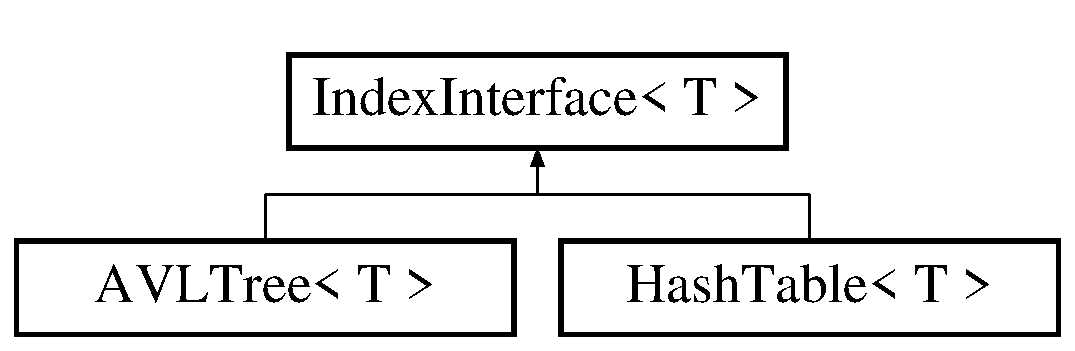
\includegraphics[height=2.000000cm]{classIndexInterface}
\end{center}
\end{figure}
\subsection*{Public Member Functions}
\begin{DoxyCompactItemize}
\item 
\mbox{\Hypertarget{classIndexInterface_ae1deeeb263b197a51d01cbf0fb16f966}\label{classIndexInterface_ae1deeeb263b197a51d01cbf0fb16f966}} 
{\bfseries Index\+Interface} (const \mbox{\hyperlink{classIndexInterface}{Index\+Interface}}$<$ T $>$ \&)
\item 
\mbox{\Hypertarget{classIndexInterface_a1894dd48debd4093c62a21e5723f4bd2}\label{classIndexInterface_a1894dd48debd4093c62a21e5723f4bd2}} 
\mbox{\hyperlink{classIndexInterface}{Index\+Interface}}$<$ T $>$ \& {\bfseries operator=} (const \mbox{\hyperlink{classIndexInterface}{Index\+Interface}}$<$ T $>$ \&)
\item 
\mbox{\Hypertarget{classIndexInterface_aec8841accbbb89e650037a64ef6bd79a}\label{classIndexInterface_aec8841accbbb89e650037a64ef6bd79a}} 
int {\bfseries get\+Num\+Questions} () const
\item 
\mbox{\Hypertarget{classIndexInterface_ac39c7591e3c5f61357c24579dfa4d5f3}\label{classIndexInterface_ac39c7591e3c5f61357c24579dfa4d5f3}} 
void {\bfseries set\+Num\+Questions} (int questions\+Indexed)
\item 
\mbox{\Hypertarget{classIndexInterface_aea1ab18b0ed842716070f3167608c8ae}\label{classIndexInterface_aea1ab18b0ed842716070f3167608c8ae}} 
virtual bool {\bfseries contains} (const T \&) const =0
\item 
\mbox{\Hypertarget{classIndexInterface_a0338c1316aff03b55aaa929071a267c5}\label{classIndexInterface_a0338c1316aff03b55aaa929071a267c5}} 
virtual std\+::pair$<$ T, bool $>$ {\bfseries search} (const T \&)=0
\item 
\mbox{\Hypertarget{classIndexInterface_ad2582c9709ab02cfb10c3f6b2da85b3f}\label{classIndexInterface_ad2582c9709ab02cfb10c3f6b2da85b3f}} 
virtual void {\bfseries insert} (const T \&)=0
\item 
\mbox{\Hypertarget{classIndexInterface_a631cf3bd60a77d52c1c7c53fc520cdad}\label{classIndexInterface_a631cf3bd60a77d52c1c7c53fc520cdad}} 
virtual bool {\bfseries is\+Empty} () const =0
\item 
\mbox{\Hypertarget{classIndexInterface_a91eb24f76a5c2d14aec1be34fb38e1ac}\label{classIndexInterface_a91eb24f76a5c2d14aec1be34fb38e1ac}} 
virtual void {\bfseries make\+Empty} ()=0
\item 
\mbox{\Hypertarget{classIndexInterface_a9fcec55df60d05560f9da1aa26b13fd9}\label{classIndexInterface_a9fcec55df60d05560f9da1aa26b13fd9}} 
virtual std\+::pair$<$ T, bool $>$ {\bfseries string\+Search} (const std\+::string \&)=0
\item 
\mbox{\Hypertarget{classIndexInterface_a6251d1376bd55e4db20d8129119d75d7}\label{classIndexInterface_a6251d1376bd55e4db20d8129119d75d7}} 
virtual void {\bfseries string\+Insert} (const std\+::string \&, int, int, int)=0
\item 
\mbox{\Hypertarget{classIndexInterface_a4897cb2ced701b463dd7d195e92ce3b4}\label{classIndexInterface_a4897cb2ced701b463dd7d195e92ce3b4}} 
virtual std\+::ostream \& {\bfseries print} (std\+::ostream \&os) const
\item 
\mbox{\Hypertarget{classIndexInterface_a41fe3e677c672edb96328a236d85dcc5}\label{classIndexInterface_a41fe3e677c672edb96328a236d85dcc5}} 
virtual std\+::vector$<$ T $>$ {\bfseries get\+Top\+Fifty} ()=0
\item 
\mbox{\Hypertarget{classIndexInterface_ad5de04ae546cb61f76ea4e3c9bf595f8}\label{classIndexInterface_ad5de04ae546cb61f76ea4e3c9bf595f8}} 
virtual int {\bfseries get\+Terms} () const =0
\end{DoxyCompactItemize}
\subsection*{Friends}
\begin{DoxyCompactItemize}
\item 
\mbox{\Hypertarget{classIndexInterface_a4576a590014d3c4b541cd772fa3efec6}\label{classIndexInterface_a4576a590014d3c4b541cd772fa3efec6}} 
std\+::ostream \& {\bfseries operator$<$$<$} (std\+::ostream \&os, const \mbox{\hyperlink{classIndexInterface}{Index\+Interface}}$<$ T $>$ \&ii)
\end{DoxyCompactItemize}


The documentation for this class was generated from the following file\+:\begin{DoxyCompactItemize}
\item 
indexinterface.\+hpp\end{DoxyCompactItemize}

\hypertarget{classinput}{}\section{input Class Reference}
\label{classinput}\index{input@{input}}
\subsection*{Public Member Functions}
\begin{DoxyCompactItemize}
\item 
\mbox{\Hypertarget{classinput_adac0ea346c43d7762baef3e3f387eebd}\label{classinput_adac0ea346c43d7762baef3e3f387eebd}} 
\mbox{\hyperlink{classinput_adac0ea346c43d7762baef3e3f387eebd}{input}} ()
\begin{DoxyCompactList}\small\item\em Prompts the user for an input Query for searching. \end{DoxyCompactList}\item 
int \mbox{\hyperlink{classinput_af8a7e9c56d11bd47067a1d6a04b97629}{get\+Flag}} ()
\begin{DoxyCompactList}\small\item\em Returns the flag that determines if words to be and/or together. \end{DoxyCompactList}\item 
vector$<$ string $>$ \mbox{\hyperlink{classinput_abc12997975bf5df011bbb073611225fa}{get\+Term\+Vector}} ()
\begin{DoxyCompactList}\small\item\em Returns the vector of terms to be searched for. \end{DoxyCompactList}\item 
vector$<$ string $>$ \mbox{\hyperlink{classinput_ac4c7f5fae89a9f8a85e05027ef1aab0d}{get\+Not\+Term\+Vector}} ()
\begin{DoxyCompactList}\small\item\em Returns the vector of terms to be notted with search results. \end{DoxyCompactList}\end{DoxyCompactItemize}
\subsection*{Public Attributes}
\begin{DoxyCompactItemize}
\item 
\mbox{\Hypertarget{classinput_a7d8969f06f1d5b287d9505db6c156fa7}\label{classinput_a7d8969f06f1d5b287d9505db6c156fa7}} 
int {\bfseries and\+Or\+Flag} = 0
\end{DoxyCompactItemize}


\subsection{Member Function Documentation}
\mbox{\Hypertarget{classinput_af8a7e9c56d11bd47067a1d6a04b97629}\label{classinput_af8a7e9c56d11bd47067a1d6a04b97629}} 
\index{input@{input}!get\+Flag@{get\+Flag}}
\index{get\+Flag@{get\+Flag}!input@{input}}
\subsubsection{\texorpdfstring{get\+Flag()}{getFlag()}}
{\footnotesize\ttfamily int input\+::get\+Flag (\begin{DoxyParamCaption}{ }\end{DoxyParamCaption})}



Returns the flag that determines if words to be and/or together. 

\begin{DoxyReturn}{Returns}
the and\+Or\+Flag used to determine if words are and-\/ed or or-\/ed together 
\end{DoxyReturn}
\mbox{\Hypertarget{classinput_ac4c7f5fae89a9f8a85e05027ef1aab0d}\label{classinput_ac4c7f5fae89a9f8a85e05027ef1aab0d}} 
\index{input@{input}!get\+Not\+Term\+Vector@{get\+Not\+Term\+Vector}}
\index{get\+Not\+Term\+Vector@{get\+Not\+Term\+Vector}!input@{input}}
\subsubsection{\texorpdfstring{get\+Not\+Term\+Vector()}{getNotTermVector()}}
{\footnotesize\ttfamily vector$<$ string $>$ input\+::get\+Not\+Term\+Vector (\begin{DoxyParamCaption}{ }\end{DoxyParamCaption})}



Returns the vector of terms to be notted with search results. 

\begin{DoxyReturn}{Returns}
the vector of not\+Words 
\end{DoxyReturn}
\mbox{\Hypertarget{classinput_abc12997975bf5df011bbb073611225fa}\label{classinput_abc12997975bf5df011bbb073611225fa}} 
\index{input@{input}!get\+Term\+Vector@{get\+Term\+Vector}}
\index{get\+Term\+Vector@{get\+Term\+Vector}!input@{input}}
\subsubsection{\texorpdfstring{get\+Term\+Vector()}{getTermVector()}}
{\footnotesize\ttfamily vector$<$ string $>$ input\+::get\+Term\+Vector (\begin{DoxyParamCaption}{ }\end{DoxyParamCaption})}



Returns the vector of terms to be searched for. 

\begin{DoxyReturn}{Returns}
the vector of and\+Or\+Words 
\end{DoxyReturn}


The documentation for this class was generated from the following files\+:\begin{DoxyCompactItemize}
\item 
input.\+h\item 
input.\+cpp\end{DoxyCompactItemize}

\hypertarget{classrunQuery}{}\section{run\+Query Class Reference}
\label{classrunQuery}\index{run\+Query@{run\+Query}}
\subsection*{Public Member Functions}
\begin{DoxyCompactItemize}
\item 
\mbox{\hyperlink{classrunQuery_aaad75dd6d53bfb24bba2ec0b7810f40a}{run\+Query}} ()
\item 
\mbox{\hyperlink{classrunQuery_aaef36fd53a33a7c44ee6ef206779dda9}{run\+Query}} (string)
\begin{DoxyCompactList}\small\item\em Searches index for and returns results of Query. \end{DoxyCompactList}\item 
pair$<$ string, string $>$ \mbox{\hyperlink{classrunQuery_a8bfd9815fef1929543a6b5b200b6a262}{delimit}} (string s)
\begin{DoxyCompactList}\small\item\em splits bracketed phrases into indivudal strings \end{DoxyCompactList}\item 
\mbox{\hyperlink{classIndexedTerm}{Indexed\+Term}} \mbox{\hyperlink{classrunQuery_ad5641a6335515ddeca95c1db2303c9b8}{bracket\+Logic}} (\mbox{\hyperlink{classIndexedTerm}{Indexed\+Term}}, \mbox{\hyperlink{classIndexedTerm}{Indexed\+Term}})
\begin{DoxyCompactList}\small\item\em Handles logic for terms which are bracketed together by and-\/ing the two indivudal terms. \end{DoxyCompactList}\item 
void \mbox{\hyperlink{classrunQuery_a19dcf052ec0adb8c4ed4df0b11094a53}{and\+Logic}} ()
\begin{DoxyCompactList}\small\item\em Handles logic to And terms together by multiplying the score of terms and-\/ed together. \end{DoxyCompactList}\item 
\mbox{\Hypertarget{classrunQuery_abd6883a84fde9aba285fa3968bdc607c}\label{classrunQuery_abd6883a84fde9aba285fa3968bdc607c}} 
void {\bfseries or\+Logic} ()
\item 
\mbox{\Hypertarget{classrunQuery_ad34874f4e2d31ee29279a4b89faaae3b}\label{classrunQuery_ad34874f4e2d31ee29279a4b89faaae3b}} 
void \mbox{\hyperlink{classrunQuery_ad34874f4e2d31ee29279a4b89faaae3b}{not\+Logic}} ()
\begin{DoxyCompactList}\small\item\em Handles logic to not terms together by modifying the score of notted terms to be very small. \end{DoxyCompactList}\end{DoxyCompactItemize}


\subsection{Constructor \& Destructor Documentation}
\mbox{\Hypertarget{classrunQuery_aaad75dd6d53bfb24bba2ec0b7810f40a}\label{classrunQuery_aaad75dd6d53bfb24bba2ec0b7810f40a}} 
\index{run\+Query@{run\+Query}!run\+Query@{run\+Query}}
\index{run\+Query@{run\+Query}!run\+Query@{run\+Query}}
\subsubsection{\texorpdfstring{run\+Query()}{runQuery()}\hspace{0.1cm}{\footnotesize\ttfamily [1/2]}}
{\footnotesize\ttfamily run\+Query\+::run\+Query (\begin{DoxyParamCaption}{ }\end{DoxyParamCaption})}

Default constructor \mbox{\Hypertarget{classrunQuery_aaef36fd53a33a7c44ee6ef206779dda9}\label{classrunQuery_aaef36fd53a33a7c44ee6ef206779dda9}} 
\index{run\+Query@{run\+Query}!run\+Query@{run\+Query}}
\index{run\+Query@{run\+Query}!run\+Query@{run\+Query}}
\subsubsection{\texorpdfstring{run\+Query()}{runQuery()}\hspace{0.1cm}{\footnotesize\ttfamily [2/2]}}
{\footnotesize\ttfamily run\+Query\+::run\+Query (\begin{DoxyParamCaption}\item[{string}]{index\+Type }\end{DoxyParamCaption})}



Searches index for and returns results of Query. 


\begin{DoxyParams}{Parameters}
{\em the} & name of the type of index to form \\
\hline
\end{DoxyParams}


\subsection{Member Function Documentation}
\mbox{\Hypertarget{classrunQuery_a19dcf052ec0adb8c4ed4df0b11094a53}\label{classrunQuery_a19dcf052ec0adb8c4ed4df0b11094a53}} 
\index{run\+Query@{run\+Query}!and\+Logic@{and\+Logic}}
\index{and\+Logic@{and\+Logic}!run\+Query@{run\+Query}}
\subsubsection{\texorpdfstring{and\+Logic()}{andLogic()}}
{\footnotesize\ttfamily void run\+Query\+::and\+Logic (\begin{DoxyParamCaption}{ }\end{DoxyParamCaption})}



Handles logic to And terms together by multiplying the score of terms and-\/ed together. 

Handles logic to Or terms together by adding the scores of terms or-\/ed together\mbox{\Hypertarget{classrunQuery_ad5641a6335515ddeca95c1db2303c9b8}\label{classrunQuery_ad5641a6335515ddeca95c1db2303c9b8}} 
\index{run\+Query@{run\+Query}!bracket\+Logic@{bracket\+Logic}}
\index{bracket\+Logic@{bracket\+Logic}!run\+Query@{run\+Query}}
\subsubsection{\texorpdfstring{bracket\+Logic()}{bracketLogic()}}
{\footnotesize\ttfamily \mbox{\hyperlink{classIndexedTerm}{Indexed\+Term}} run\+Query\+::bracket\+Logic (\begin{DoxyParamCaption}\item[{\mbox{\hyperlink{classIndexedTerm}{Indexed\+Term}}}]{t1,  }\item[{\mbox{\hyperlink{classIndexedTerm}{Indexed\+Term}}}]{t2 }\end{DoxyParamCaption})}



Handles logic for terms which are bracketed together by and-\/ing the two indivudal terms. 


\begin{DoxyParams}{Parameters}
{\em the} & first \mbox{\hyperlink{classIndexedTerm}{Indexed\+Term}} of the bracketed phrase \\
\hline
{\em the} & second \mbox{\hyperlink{classIndexedTerm}{Indexed\+Term}} of the bracketed phrase \\
\hline
\end{DoxyParams}
\begin{DoxyReturn}{Returns}
an Indexed phrase holding all the question\+I\+Ds the terms share with inflated frequencies 
\end{DoxyReturn}
\mbox{\Hypertarget{classrunQuery_a8bfd9815fef1929543a6b5b200b6a262}\label{classrunQuery_a8bfd9815fef1929543a6b5b200b6a262}} 
\index{run\+Query@{run\+Query}!delimit@{delimit}}
\index{delimit@{delimit}!run\+Query@{run\+Query}}
\subsubsection{\texorpdfstring{delimit()}{delimit()}}
{\footnotesize\ttfamily pair$<$ string, string $>$ run\+Query\+::delimit (\begin{DoxyParamCaption}\item[{string}]{s }\end{DoxyParamCaption})}



splits bracketed phrases into indivudal strings 


\begin{DoxyParams}{Parameters}
{\em the} & string to split into two strings \\
\hline
\end{DoxyParams}
\begin{DoxyReturn}{Returns}
a pair of strings containing each term 
\end{DoxyReturn}


The documentation for this class was generated from the following files\+:\begin{DoxyCompactItemize}
\item 
runquery.\+h\item 
runquery.\+cpp\end{DoxyCompactItemize}

\hypertarget{classSearchEngine}{}\section{Search\+Engine Class Reference}
\label{classSearchEngine}\index{Search\+Engine@{Search\+Engine}}
\subsection*{Public Member Functions}
\begin{DoxyCompactItemize}
\item 
\mbox{\Hypertarget{classSearchEngine_a1808d0f69adc101d7b6847f4ac13a970}\label{classSearchEngine_a1808d0f69adc101d7b6847f4ac13a970}} 
void {\bfseries run} ()
\end{DoxyCompactItemize}


The documentation for this class was generated from the following files\+:\begin{DoxyCompactItemize}
\item 
searchengine.\+h\item 
searchengine.\+cpp\end{DoxyCompactItemize}

\chapter{File Documentation}
\hypertarget{porter2__stemmer_8cpp}{}\section{porter2\+\_\+stemmer.\+cpp File Reference}
\label{porter2__stemmer_8cpp}\index{porter2\+\_\+stemmer.\+cpp@{porter2\+\_\+stemmer.\+cpp}}
{\ttfamily \#include $<$algorithm$>$}\newline
{\ttfamily \#include $<$utility$>$}\newline
{\ttfamily \#include $<$unordered\+\_\+map$>$}\newline
{\ttfamily \#include \char`\"{}porter2\+\_\+stemmer.\+h\char`\"{}}\newline


\subsection{Detailed Description}
\begin{DoxyAuthor}{Author}
Sean Massung 
\end{DoxyAuthor}
\begin{DoxyDate}{Date}
September 2012
\end{DoxyDate}
Implementation of \href{http://snowball.tartarus.org/algorithms/english/stemmer.html}{\tt http\+://snowball.\+tartarus.\+org/algorithms/english/stemmer.\+html}

Copyright (C) 2012 Sean Massung

Permission is hereby granted, free of charge, to any person obtaining a copy of this software and associated documentation files (the \char`\"{}\+Software\char`\"{}), to deal in the Software without restriction, including without limitation the rights to use, copy, modify, merge, publish, distribute, sublicense, and/or sell copies of the Software, and to permit persons to whom the Software is furnished to do so, subject to the following conditions\+:

The above copyright notice and this permission notice shall be included in all copies or substantial portions of the Software.

T\+HE S\+O\+F\+T\+W\+A\+RE IS P\+R\+O\+V\+I\+D\+ED \char`\"{}\+A\+S I\+S\char`\"{}, W\+I\+T\+H\+O\+UT W\+A\+R\+R\+A\+N\+TY OF A\+NY K\+I\+ND, E\+X\+P\+R\+E\+SS OR I\+M\+P\+L\+I\+ED, I\+N\+C\+L\+U\+D\+I\+NG B\+UT N\+OT L\+I\+M\+I\+T\+ED TO T\+HE W\+A\+R\+R\+A\+N\+T\+I\+ES OF M\+E\+R\+C\+H\+A\+N\+T\+A\+B\+I\+L\+I\+TY, F\+I\+T\+N\+E\+SS F\+OR A P\+A\+R\+T\+I\+C\+U\+L\+AR P\+U\+R\+P\+O\+SE A\+ND N\+O\+N\+I\+N\+F\+R\+I\+N\+G\+E\+M\+E\+NT. IN NO E\+V\+E\+NT S\+H\+A\+LL T\+HE A\+U\+T\+H\+O\+RS OR C\+O\+P\+Y\+R\+I\+G\+HT H\+O\+L\+D\+E\+RS BE L\+I\+A\+B\+LE F\+OR A\+NY C\+L\+A\+IM, D\+A\+M\+A\+G\+ES OR O\+T\+H\+ER L\+I\+A\+B\+I\+L\+I\+TY, W\+H\+E\+T\+H\+ER IN AN A\+C\+T\+I\+ON OF C\+O\+N\+T\+R\+A\+CT, T\+O\+RT OR O\+T\+H\+E\+R\+W\+I\+SE, A\+R\+I\+S\+I\+NG F\+R\+OM, O\+UT OF OR IN C\+O\+N\+N\+E\+C\+T\+I\+ON W\+I\+TH T\+HE S\+O\+F\+T\+W\+A\+RE OR T\+HE U\+SE OR O\+T\+H\+ER D\+E\+A\+L\+I\+N\+GS IN T\+HE S\+O\+F\+T\+W\+A\+RE. 
\hypertarget{porter2__stemmer_8h}{}\section{porter2\+\_\+stemmer.\+h File Reference}
\label{porter2__stemmer_8h}\index{porter2\+\_\+stemmer.\+h@{porter2\+\_\+stemmer.\+h}}
{\ttfamily \#include $<$vector$>$}\newline
{\ttfamily \#include $<$string$>$}\newline
{\ttfamily \#include \char`\"{}util/string\+\_\+view.\+h\char`\"{}}\newline
\subsection*{Functions}
\begin{DoxyCompactItemize}
\item 
\mbox{\Hypertarget{porter2__stemmer_8h_ad07c4652a1144329db4bdfb6ce640d80}\label{porter2__stemmer_8h_ad07c4652a1144329db4bdfb6ce640d80}} 
void {\bfseries Porter2\+Stemmer\+::stem} (std\+::string \&word)
\item 
\mbox{\Hypertarget{porter2__stemmer_8h_ac74222c2eb041cff861fddfd529bc983}\label{porter2__stemmer_8h_ac74222c2eb041cff861fddfd529bc983}} 
void {\bfseries Porter2\+Stemmer\+::trim} (std\+::string \&word)
\item 
\mbox{\Hypertarget{porter2__stemmer_8h_a4419080bc3b64aca4998a732e9f99d84}\label{porter2__stemmer_8h_a4419080bc3b64aca4998a732e9f99d84}} 
size\+\_\+t {\bfseries Porter2\+Stemmer\+::internal\+::first\+Non\+Vowel\+After\+Vowel} (const std\+::string \&word, size\+\_\+t start)
\item 
\mbox{\Hypertarget{porter2__stemmer_8h_a2d7e133e04950f30c9b3a2935be7c802}\label{porter2__stemmer_8h_a2d7e133e04950f30c9b3a2935be7c802}} 
size\+\_\+t {\bfseries Porter2\+Stemmer\+::internal\+::get\+Start\+R1} (const std\+::string \&word)
\item 
\mbox{\Hypertarget{porter2__stemmer_8h_a87bb0a5733b6267185b7951349477070}\label{porter2__stemmer_8h_a87bb0a5733b6267185b7951349477070}} 
size\+\_\+t {\bfseries Porter2\+Stemmer\+::internal\+::get\+Start\+R2} (const std\+::string \&word, size\+\_\+t start\+R1)
\item 
\mbox{\Hypertarget{porter2__stemmer_8h_add0f2aec57b66845cb78e98844bb4205}\label{porter2__stemmer_8h_add0f2aec57b66845cb78e98844bb4205}} 
void {\bfseries Porter2\+Stemmer\+::internal\+::changeY} (std\+::string \&word)
\item 
\mbox{\Hypertarget{porter2__stemmer_8h_ae689551ae90968445d4ab1a60ffc805c}\label{porter2__stemmer_8h_ae689551ae90968445d4ab1a60ffc805c}} 
void {\bfseries Porter2\+Stemmer\+::internal\+::step0} (std\+::string \&word)
\item 
\mbox{\Hypertarget{porter2__stemmer_8h_af0acc908e606cd6e2917bf2ed31d5fe7}\label{porter2__stemmer_8h_af0acc908e606cd6e2917bf2ed31d5fe7}} 
bool {\bfseries Porter2\+Stemmer\+::internal\+::step1A} (std\+::string \&word)
\item 
\mbox{\Hypertarget{porter2__stemmer_8h_af4cffda4b443475c766407d60eac03dc}\label{porter2__stemmer_8h_af4cffda4b443475c766407d60eac03dc}} 
void {\bfseries Porter2\+Stemmer\+::internal\+::step1B} (std\+::string \&word, size\+\_\+t start\+R1)
\item 
\mbox{\Hypertarget{porter2__stemmer_8h_abc52eb93a0acc99087ca62bb2a4e647e}\label{porter2__stemmer_8h_abc52eb93a0acc99087ca62bb2a4e647e}} 
void {\bfseries Porter2\+Stemmer\+::internal\+::step1C} (std\+::string \&word)
\item 
\mbox{\Hypertarget{porter2__stemmer_8h_a8bde57d3eeee683082f53cd7a9a0a2f8}\label{porter2__stemmer_8h_a8bde57d3eeee683082f53cd7a9a0a2f8}} 
void {\bfseries Porter2\+Stemmer\+::internal\+::step2} (std\+::string \&word, size\+\_\+t start\+R1)
\item 
\mbox{\Hypertarget{porter2__stemmer_8h_a8ea5872c398ea38fb5ff359879613a4e}\label{porter2__stemmer_8h_a8ea5872c398ea38fb5ff359879613a4e}} 
void {\bfseries Porter2\+Stemmer\+::internal\+::step3} (std\+::string \&word, size\+\_\+t start\+R1, size\+\_\+t start\+R2)
\item 
\mbox{\Hypertarget{porter2__stemmer_8h_a46c7932444166421508feab27b1addfa}\label{porter2__stemmer_8h_a46c7932444166421508feab27b1addfa}} 
void {\bfseries Porter2\+Stemmer\+::internal\+::step4} (std\+::string \&word, size\+\_\+t start\+R2)
\item 
\mbox{\Hypertarget{porter2__stemmer_8h_ad53abf614a24cba562dba83857f42091}\label{porter2__stemmer_8h_ad53abf614a24cba562dba83857f42091}} 
void {\bfseries Porter2\+Stemmer\+::internal\+::step5} (std\+::string \&word, size\+\_\+t start\+R1, size\+\_\+t start\+R2)
\item 
\mbox{\Hypertarget{porter2__stemmer_8h_a15dc6085d05bf8e2ee691ef08e0fae29}\label{porter2__stemmer_8h_a15dc6085d05bf8e2ee691ef08e0fae29}} 
bool {\bfseries Porter2\+Stemmer\+::internal\+::is\+Short} (const std\+::string \&word)
\item 
\mbox{\Hypertarget{porter2__stemmer_8h_a7c20680dfe258c8050c8225d97b2e160}\label{porter2__stemmer_8h_a7c20680dfe258c8050c8225d97b2e160}} 
bool {\bfseries Porter2\+Stemmer\+::internal\+::special} (std\+::string \&word)
\item 
\mbox{\Hypertarget{porter2__stemmer_8h_a63d428e12b7b2aeea945c24afe44d1d2}\label{porter2__stemmer_8h_a63d428e12b7b2aeea945c24afe44d1d2}} 
bool {\bfseries Porter2\+Stemmer\+::internal\+::is\+Vowel} (char ch)
\item 
\mbox{\Hypertarget{porter2__stemmer_8h_a72ec1ef1732191be64f203bbe0e4397d}\label{porter2__stemmer_8h_a72ec1ef1732191be64f203bbe0e4397d}} 
bool {\bfseries Porter2\+Stemmer\+::internal\+::is\+VowelY} (char ch)
\item 
\mbox{\Hypertarget{porter2__stemmer_8h_a28eb8ebf000d316d4a047a0a55abab7d}\label{porter2__stemmer_8h_a28eb8ebf000d316d4a047a0a55abab7d}} 
bool {\bfseries Porter2\+Stemmer\+::internal\+::ends\+With} (meta\+::util\+::string\+\_\+view word, meta\+::util\+::string\+\_\+view str)
\item 
\mbox{\Hypertarget{porter2__stemmer_8h_aca68167dfec7979b35d5bc732d2c6ef0}\label{porter2__stemmer_8h_aca68167dfec7979b35d5bc732d2c6ef0}} 
bool {\bfseries Porter2\+Stemmer\+::internal\+::ends\+In\+Double} (const std\+::string \&word)
\item 
\mbox{\Hypertarget{porter2__stemmer_8h_ad6f95ce8820c7f829d0f0707ee437480}\label{porter2__stemmer_8h_ad6f95ce8820c7f829d0f0707ee437480}} 
bool {\bfseries Porter2\+Stemmer\+::internal\+::replace\+If\+Exists} (std\+::string \&word, meta\+::util\+::string\+\_\+view suffix, meta\+::util\+::string\+\_\+view replacement, size\+\_\+t start)
\item 
\mbox{\Hypertarget{porter2__stemmer_8h_acb88f8cc716be69a9c19818473614d68}\label{porter2__stemmer_8h_acb88f8cc716be69a9c19818473614d68}} 
bool {\bfseries Porter2\+Stemmer\+::internal\+::is\+Valid\+L\+I\+Ending} (char ch)
\item 
\mbox{\Hypertarget{porter2__stemmer_8h_ade420031f6e4e4a9f432c82b7f54420b}\label{porter2__stemmer_8h_ade420031f6e4e4a9f432c82b7f54420b}} 
bool {\bfseries Porter2\+Stemmer\+::internal\+::contains\+Vowel} (const std\+::string \&word, size\+\_\+t start, size\+\_\+t end)
\end{DoxyCompactItemize}


\subsection{Detailed Description}
\begin{DoxyAuthor}{Author}
Sean Massung 
\end{DoxyAuthor}
\begin{DoxyDate}{Date}
September 2012
\end{DoxyDate}
Implementation of \href{http://snowball.tartarus.org/algorithms/english/stemmer.html}{\tt http\+://snowball.\+tartarus.\+org/algorithms/english/stemmer.\+html}

Copyright (C) 2012 Sean Massung

Permission is hereby granted, free of charge, to any person obtaining a copy of this software and associated documentation files (the \char`\"{}\+Software\char`\"{}), to deal in the Software without restriction, including without limitation the rights to use, copy, modify, merge, publish, distribute, sublicense, and/or sell copies of the Software, and to permit persons to whom the Software is furnished to do so, subject to the following conditions\+:

The above copyright notice and this permission notice shall be included in all copies or substantial portions of the Software.

T\+HE S\+O\+F\+T\+W\+A\+RE IS P\+R\+O\+V\+I\+D\+ED \char`\"{}\+A\+S I\+S\char`\"{}, W\+I\+T\+H\+O\+UT W\+A\+R\+R\+A\+N\+TY OF A\+NY K\+I\+ND, E\+X\+P\+R\+E\+SS OR I\+M\+P\+L\+I\+ED, I\+N\+C\+L\+U\+D\+I\+NG B\+UT N\+OT L\+I\+M\+I\+T\+ED TO T\+HE W\+A\+R\+R\+A\+N\+T\+I\+ES OF M\+E\+R\+C\+H\+A\+N\+T\+A\+B\+I\+L\+I\+TY, F\+I\+T\+N\+E\+SS F\+OR A P\+A\+R\+T\+I\+C\+U\+L\+AR P\+U\+R\+P\+O\+SE A\+ND N\+O\+N\+I\+N\+F\+R\+I\+N\+G\+E\+M\+E\+NT. IN NO E\+V\+E\+NT S\+H\+A\+LL T\+HE A\+U\+T\+H\+O\+RS OR C\+O\+P\+Y\+R\+I\+G\+HT H\+O\+L\+D\+E\+RS BE L\+I\+A\+B\+LE F\+OR A\+NY C\+L\+A\+IM, D\+A\+M\+A\+G\+ES OR O\+T\+H\+ER L\+I\+A\+B\+I\+L\+I\+TY, W\+H\+E\+T\+H\+ER IN AN A\+C\+T\+I\+ON OF C\+O\+N\+T\+R\+A\+CT, T\+O\+RT OR O\+T\+H\+E\+R\+W\+I\+SE, A\+R\+I\+S\+I\+NG F\+R\+OM, O\+UT OF OR IN C\+O\+N\+N\+E\+C\+T\+I\+ON W\+I\+TH T\+HE S\+O\+F\+T\+W\+A\+RE OR T\+HE U\+SE OR O\+T\+H\+ER D\+E\+A\+L\+I\+N\+GS IN T\+HE S\+O\+F\+T\+W\+A\+RE. 
%--- End generated contents ---

% Index
\backmatter
\newpage
\phantomsection
\clearemptydoublepage
\addcontentsline{toc}{chapter}{Index}
\printindex

\end{document}
